\documentclass[machines,article,submit,pdftex,moreauthors]{Definitions/mdpi}

\pdftrailerid{}
\pdfsuppressptexinfo=15
\graphicspath{{figures/}}

\soulregister\eqref7
\soulregister\ref7

\AtBeginDocument{\pdfstringdefDisableCommands{\def\hl#1{#1}\def\textls[#1]#2{#2}\def\colorbox#1#2{#2}}}


















\firstpage{1}
\makeatletter
\setcounter{page}{\@firstpage}
\makeatother
\pubvolume{14}
\issuenum{11}
\articlenumber{1248}
\pubyear{2026}
\copyrightyear{2026}
\externaleditor{Carmine Maria Pappalardo}
\datereceived{9 October 2026}
\daterevised{21 October 2026}
\dateaccepted{21 October 2026}
\datepublished{24 October 2026}


\hreflink{https://doi.org/10.3390/machines14111248}


\Title{Observer-Based Hybrid Position Holding for an Electrohydraulic Agricultural Hitch: A Two-Chamber Virtual-Prototype Stress Test}
\newcommand{\orcidauthorA}{0009-0005-1928-6218}
\Author{Chenyu Cui\orcidA{}
, Peng Wang and Yucheng Zhang
 *}
\AuthorNames{Chenyu Cui, Peng Wang and Yucheng Zhang}


\address[1]{Prospective Research Laboratory,
 Institute of Computing Technology, Chinese Academy of Sciences, \linebreak  Beijing 100190, China; cuichenyu25s@ict.ac.cn (C.C.); wangpeng2021@ict.ac.cn (P.W.)
}




\corres{\hangafter=1 \hangindent=1.0em \hspace{-1em} Correspondence: zhangyucheng@ict.ac.cn}







\abstract{Electrohydraulic holding is evaluated as a trade-off between accuracy, main-source throughput and finite storage. A symmetric virtual plant represents chamber pressures, spool lag, leakage, friction and gas storage. Component ablations and equal-budget comparisons distinguish sensing, dwell and controller effects. Corrected active sliding-mode control has lower nominal means on the four previously evaluated objectives than the earlier hybrids. A separate resource-oriented search gives each policy nine gain pairs and three complete development paths. On four independent normal-supply validation seeds, the selected hybrid/sliding-mode boundary resource is 22.47/209.32 kJ, with RMSE \mbox{1.208/0.309 mm}; both pass the declared 10 mm screen. Chamber continuity explains why stationary piston/pressure holding during supply disconnection requires storage inflow and a return path. A separately frozen 88-path study includes eight new joint parameter/sensing vectors with a 1200 s supply interruption in 1800 s simulations. Scalar and availability-aware hybrids each pass 8/8 with storage and 1/8 without under the declared error/drop screens. The availability rule reduces mean within-interruption maximum error from 3.571 to \mbox{1.173 mm} while increasing mean storage use from 286.68 to 409.74 mL. Both-port-blocked failures remain archived. These conditional theoretical results establish neither total-energy savings, globally resource-optimal tuning, physical reliability nor global nonlinear stability.}
\keyword{\textls[-20]{agricultural machinery; electrohydraulic actuator; two-chamber model; three-point} hitch; position holding; interface observer; virtual prototype; hybrid supervision}
\begin{document}

\section{Introduction}
Rear hitches must accomplish two tasks with fundamentally different time scales: move an implement to a commanded position and maintain that position after motion has ended. Position holding is not merely the final portion of a tracking transient. It governs implement-depth retention, hydraulic energy consumption, and~valve activity while the tractor operates under a quasi-static load. During~this phase, cylinder and lock-valve leakage, load changes, temperature, sensor noise, and~the available hydraulic storage can all produce a slow position drift. A~controller optimized only for tracking can therefore generate unnecessary valve activity or fail to distinguish a persistent loss path from a transient~disturbance.

Tool design also influences the operating conditions that hitch control seeks to maintain. Syromyatnikov~et~al. studied flat-blade parameters for soil loosening~\cite{syromyatnikov2022}, and~examined tillage-quality indicators for a unit with a flexible working body~\cite{syromyatnikov2023}. These studies motivate attention to implement working conditions, but~do not establish a quantitative relation between the present virtual holding error and soil quality. This study evaluates actuator position; soil--tool interaction and agronomic outcomes are outside its~model.

The practical importance of this distinction is increasing as tractor hitches are integrated with automated depth control and coordinated traction functions. A~recent review of tractor electrohydraulic hitch systems documents the breadth of position, draft, and~mixed-control architectures used in agricultural machinery~\cite{sun2022}. At~the component level, the~flow characteristics of a tractor electrohydraulic hitch valve have been modeled and experimentally validated~\cite{kumar2021}; at the system level, coordinated hitch-depth and travel-speed control has been studied as an efficiency-oriented agricultural operation~\cite{sun2025}. These studies motivate a clear representation of the hydraulic and supervisory mechanisms that govern a transition from commanded motion to~holding.

Recent tractor research has also reported hitch-position estimation using an EKF--Transformer architecture~\cite{kim2025} and robust draft/position control with differential and integral sliding modes~\cite{liu2023}. More generally, electrohydraulic servo research provides established sliding-mode and adaptive-control designs~\cite{bai2010,tang2011,jin2013}. These contributions establish useful control ingredients, but~their performance evidence has different objectives from a long-hold stress test: many studies emphasize trajectory tracking, draft regulation, or~a specific hardware configuration rather than the entry logic, retained leakage path, and~storage-assisted response during an extended~hold.

For a holding study, the~evaluation protocol must be distinguished from any claim of physical performance. A~small average drop can arise because a controller has not entered its hold mode, because~the disturbance is unrealistically smooth, or~because a noise-free internal pressure state is available to the controller. Conversely, a~conservative velocity gate can prevent hold entry even when position tracking is stable. Reporting the entry criterion, time horizon, load disturbance, and~parameter range is therefore as important as reporting position error. Simulation verification and physical validation address different questions~\cite{sargent2013}: repeatable seeded noise can test a model's internal behavior, but~cannot establish the performance of a hydraulic~machine.

This work investigates conditional holding performance under noisy position and chamber-pressure sensing. The~original control chains use those measurements and a shared observer to coordinate tracking, bounded trim, locking and finite accumulator compensation. A~separate availability experiment also provides the current ideal supply-status flag to every comparator and tests an availability-aware extension. The~virtual prototype exposes its loss paths, pressure interface, mode transitions, parameter classes and stress inputs. Its results concern the specified theoretical plant, with~numerical verification separated from physical~validation.

\section{Related~Work}
\unskip
\subsection{Hitch Control and Electrohydraulic Motion~Regulation}
Research on tractor hitches covers system development, coordination of agricultural operations, and~actuator control. Reviews describe the sensing and hydraulic architectures used in position, draft, and~mixed control~\cite{sun2022}. Valve-flow studies provide component-specific experimental evidence~\cite{kumar2021}, while coordinated depth and speed control links hitch commands to operating efficiency~\cite{sun2025}. Tractor-specific sliding-mode control~\cite{liu2023} and hitch-position estimation~\cite{kim2025} address complementary regulation and sensing tasks. These sources establish the application context; their measurements are not used to calibrate the virtual prototype in this~study.

Hydraulic servo models describe the coupling between flow, pressure, mechanical load, and~displacement~\cite{jelali2003}. Adaptive robust motion control of hydraulic actuators~\cite{yao2000}, adaptive sliding-mode control with unknown parameters~\cite{guan2008}, and~nonlinear adaptive suspension control~\cite{alleyne1995} provide established approaches to nonlinear regulation. Force control requires attention to the pressure--load relationship~\cite{alleyne2000}, while backstepping designs can explicitly include valve dynamics~\cite{choux2010}. Valve dead-zone compensation is another distinct source of motion-control improvement~\cite{deng2017}. These methods inform the actuator-level context, but~a comparison of tracking error alone does not evaluate long-duration hold entry, switching activity, and~finite stored-fluid~use.

Hydraulic switching has also been used to supplement speed-variable drives. Zagar~et~al. reported a switching architecture that combines discrete hydraulic paths with a variable-speed drive and evaluated its effect on the drive operating point and efficiency

~\cite{zagar2020}. That study provides a useful comparison for the present supervisor because both approaches use discrete hydraulic decisions to reduce the burden on a continuously actuated path. The~present contribution addresses a different question: whether a noisy, observer-based supervisor can coordinate TRACK, FINE\_TRIM, LOCK, and~finite-accumulator support during a 30 min holding protocol. The~comparison is therefore at the level of supervisory objective and evidence, rather than a claim that the two virtual or physical drive architectures are~interchangeable.

Recent studies also illustrate the diversity of electrohydraulic control problems. Feng~et~al. combined disturbance observation with sliding-mode spool-position control~\cite{feng2025}. Wang and Song studied clearance compensation using a Hopfield neural network~\cite{wang2024}, and~Hanaffi~et~al. evaluated optimized fractional-order PID position tracking through hardware-in-the-loop implementation~\cite{hanaffi2026}. Their objectives and validation settings differ from the present 30 min holding protocol. The~original comparisons use complete PID--lock, sliding-mode--lock, and~PID--accumulator control chains. A~follow-up adds an active sliding-mode chain with the same sensing, holding authority and development budget. These comparisons evaluate the specified supervisory problem without establishing superiority over all actuator-level control~methods.

\subsection{Observation, Hydraulic Storage, and~Mode~Supervision}
Disturbance-observer-based control~\cite{chen2016} and active disturbance rejection~\cite{han2009} provide a broader context for estimating unmeasured effects from controller-facing signals. Hydraulic leakage detection using an extended Kalman filter is a related diagnostic problem~\cite{an2005}; it should be distinguished from reconstructing an internal coefficient from an exact virtual-model transition. Here, velocity and effective-load estimates enter the V2 control law, whereas a residual-based leakage diagnostic is unused by feedback and is not identified with a physical leakage coefficient. The~earlier reduced-order leakage proxy is retained separately to make this distinction~explicit.

Low-speed behavior also depends on mechanical and fluid assumptions. Friction modeling and compensation are well-established topics~\cite{wit1995,olsson1998}, and~experimental work shows that an oil--air mixture's effective bulk modulus depends on its physical conditions~\cite{gholizadeh2013}. Reviews of pump-controlled cylinder drives further show why actuator architecture matters when interpreting hydraulic efficiency~\cite{ketelsen2019}. The~present valve-controlled model uses researcher-defined friction, bulk-modulus, leakage, and~accumulator inputs. Accordingly, reduced accumulator-oil use is reported as a controller-activity metric; it is not converted into an unmeasured system-energy~saving.

Hybrid-system theory separates continuous dynamics from discrete mode transitions~\cite{goebel2009}. Stability analyses of switched systems~\cite{liberzon1999} and average dwell time~\cite{hespanha1999} motivate explicit switching rules, but~a numerical minimum dwell time alone does not prove closed-loop stability. In~this study, hysteresis and an 8 s dwell constraint limit mode activity in the evaluated simulations. The~analysis distinguishes a corrected legacy coefficient-proxy bound, bounded states of the projected numerical V2 model, and~a local frozen-volume mode analysis. None is a global stability guarantee for the nonlinear switched \mbox{hydraulic~system}.

\subsection{Scope of the Present~Contribution}
The contribution is the coordination and evaluation of low-activity holding modes under a shared measurement interface. The~primary plant maintains separate chamber-pressure states, finite accumulator storage, and~explicit spool and pressure limits. The~original four control chains share the observer and nominal tracking bandwidth. Supervisor selection on five development seeds is separated from 20 frozen holdout runs, and~adverse sensor-bias outcomes remain in the results. Follow-up development specifies a common gain grid, objective and control authority for active comparisons, with~an explicitly separate accuracy-margin choice. Following the distinction between verification and validation~\cite{sargent2013}, the~evidence concerns the specified virtual prototype. The~deterministic stress tests examine selected perturbations; they do not estimate variance-based sensitivity indices or a physical failure probability~\cite{saltelli2010}.

The experiments ask four specific questions. First, which changes in holding arise from the filtered measurement/load interface, and~which arise from dwell and discharge gating? Crossed interface removals and matched-timer controls address that attribution. Second, after~equal development effort and holding authority are imposed, which of drop, tracking error, stored-fluid use and mode activity improve or deteriorate? The active-policy comparisons retain every objective and failed path. Third, does a development accuracy reserve remove sampled transition failures on a new simultaneous uncertainty design, and~what fluid-use cost does it impose? Fourth, how does actual main-supply throughput change the resource--tracking comparison, and~when does storage contribute under a declared supply restriction? A separate frozen availability study tests a necessary chamber-flow balance and an availability-conditioned hybrid rule. These questions define an evaluation contribution; the observer recursions and boundary-layer sliding term are established ingredients rather than new estimation or robust-control~theorems.


\section{Materials and~Methods}
\unskip
\subsection{Two-Chamber Virtual Plant and Modeling~Boundary}
\label{sec3.1}

The primary V2 model has separate chamber pressures, piston position and velocity, spool position, and~accumulator gas volume. All coefficients are declared theoretical~inputs.



The schematic makes the modeling boundary explicit. The~cylinder coordinate $x$ is the simulated piston displacement. If~a physical linkage were introduced, implement displacement would require a geometry-dependent map such as $\Delta z_i=G_\ell(x)\Delta x$; therefore, the reported 10 mm screen is a cylinder-coordinate criterion and is not interpreted as a calibrated implement-depth~error.

With $A=0.012$ m$^2$, $V_0=0.004$ m$^3$, effective bulk modulus $\beta_e=0.20$ GPa and stroke $L=0.85$ m, the~chamber volumes are $V_A=V_0+Ax$ and $V_B=V_0+A(L-x)$. The~implemented continuity equations are given in Equation~\eqref{eq:continuity}

\begin{equation}
\dot p_A=\frac{\beta_e}{V_A}(q_A+q_{acc}-Av-q_l),\quad
\dot p_B=\frac{\beta_e}{V_B}(Av-q_B+q_l),\quad
q_l=C_l(T)(p_A-p_B).
\label{eq:continuity}
\end{equation}

Here,

 $C_l(T)=C_{l,25}[1+0.018\max(T-25,0)]$, with~$C_{l,25}=5\times10^{-14}$ m$^3$ s$^{-1}$ Pa$^{-1}$. Each term inside a parenthesis is a volume flow in m$^3$ s$^{-1}$ and each pressure derivative is in \mbox{Pa s$^{-1}$}. Mechanical motion satisfies Equation~\eqref{eq:mechanical}
\begin{equation}
m\dot v=A(p_A-p_B)-F_L-kx-cv-F_d(v),\qquad \dot x=v,
\label{eq:mechanical}
\end{equation}
where $m=1200$ kg, $k=18000$ N m$^{-1}$, $c=2200$ N s m$^{-1}$, and~$F_d(v)=\operatorname{sgn}(v)[850+350\max(1-|v|/0.004,0)]$ N. The~code sets the sign to zero for $|v|<10^{-7}$ m s$^{-1}$; it does not solve a set-valued static-friction~law.

Equal chamber areas define a symmetric virtual actuator. They do not describe the geometry of a conventional single-rod hitch cylinder. For~a single rod, $A_A\ne A_B$, the~force becomes $A_Ap_A-A_Bp_B$, volumes become $V_{A0}+A_Ax$ and $V_{B0}+A_B(L-x)$, and~the pressure-balance target and observer must also change~\cite{yao2000,ketelsen2019}. Those changes affect available force, flow demand, common-pressure coupling, and~accumulator discharge. We retain symmetry to isolate supervisory mechanisms under a single declared plant; no transfer of the reported millimeter results to an asymmetric cylinder is~assumed.

The spool obeys $\dot z=(u-z)/0.05$ with $u\in[-1,1]$. Its effective opening is $a=5\times10^{-6}\max[(|z|-0.03)/0.97,0]$ m$^2$. Define $Q(a,\Delta p)=0.62a\sqrt{2\max(\Delta p,0)/850}$. For~$z\ge0$, $(q_A,q_B)=(Q(a,p_s-p_A),Q(a,p_B-p_t))$; for $z<0$, $(q_A,q_B)=(-Q(a,p_A-p_t),-Q(a,p_s-p_B))$. Supply, tank, and~relief pressures are 21, 0.2, and~22 MPa. Pressures are projected to $[p_t,p_{rel}]$ after every numerical integration substep; stroke exits are projected and velocity is reset. These projections are numerical boundary rules, not modeled relief-flow or cavitation dynamics. Likewise, the~lock symbols in Figure~\ref{fig:physical-system} represent a supervisory shut-off request implemented by $u=0$. V2 has no independent lock-valve state or pilot/check-valve flow law: the spool settles through its stated lag, and~internal leakage remains active in LOCK. The~drawing is therefore a hydraulic abstraction rather than a component-complete hardware~circuit.


\begin{figure}[H]

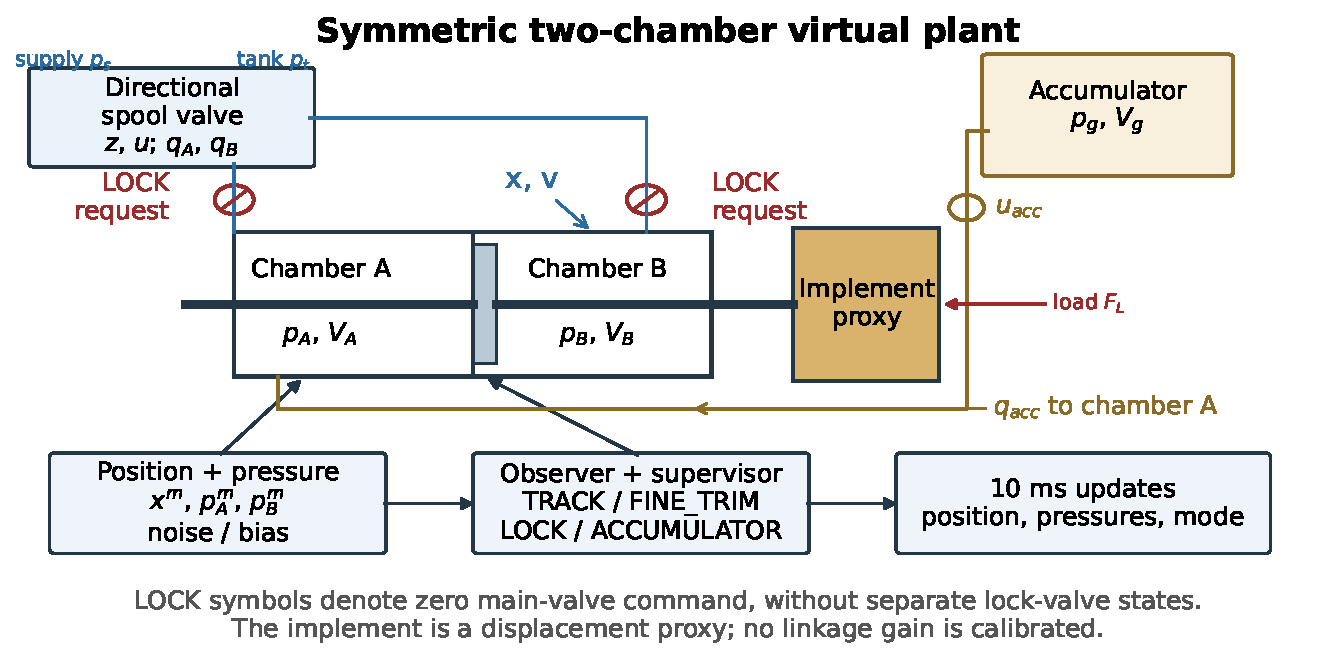
\includegraphics[width=\linewidth]{reviewer3_physical_system.pdf}
\caption{Hydraulic
 abstraction for the symmetric two-chamber virtual plant. The~directional spool valve, finite accumulator, piston/rod and implement displacement proxy are connected to the measured signals and 10 ms observer--supervisor interface. LOCK symbols denote a zero main-valve command, not separately modeled lock-valve dynamics. No linkage gain is~calibrated.}
\label{fig:physical-system}
\end{figure}


The finite accumulator uses $p_gV_g^{1.2}=\mathrm{constant}$, shell volume 4 L, precharge 8 MPa, and~initial pressure 14 MPa. Its discharge is $q_{acc}=u_{acc}5\times10^{-8}\sqrt{\max(p_g-p_A,0)}$, capped by available oil per integration step, and~$\dot V_g=q_{acc}$. The~coefficient has units m$^3$ s$^{-1}$ Pa$^{-1/2}$; $u_{acc}$ is dimensionless and $q_{acc}$ is in m$^3$ s$^{-1}$. There is no recharge branch in V2. Initial chamber common pressure is 5 MPa, the~initial differential balances the 9 kN load and spring at $x=0.15$ m, and~initial velocity and spool are zero. The~full original parameter manifest and the separate revision-override ledger accompany the~code. The archived nonlinear-comparison execution environment records Python 3.9.6, NumPy 2.0.2 and SciPy 1.13.1. No physical equipment was used.

\subsection{Measurement Interface and Implemented~Observer}
At controller period $h_c=0.01$ s, the measured position and two measured pressures contain independent zero-mean Gaussian samples with standard deviations 1.5 mm and 0.05 MPa, respectively. Bias and noise changes are explicit stress inputs. Let $r_k=x^m_k-\hat x_k$. In~the order used by the code, Equations~\eqref{eq:observer-position}--\eqref{eq:observer} give the updates:
\begin{align}
\hat x_{k+1}&=\hat x_k+h_c\hat v_k+0.08r_k,&
\hat v_{k+1}&=\hat v_k+(0.0005/h_c)r_k,\label{eq:observer-position}\\
\hat p_{j,k+1}&=\hat p_{j,k}+0.18(p^m_{j,k}-\hat p_{j,k}),&j&\in\{A,B\},\label{eq:observer-pressure}\\
\hat a_k&=(\hat v_{k+1}-\hat v_k)/h_c,&
F_k^{raw}&=A(\hat p_{A,k+1}-\hat p_{B,k+1})-k\hat x_{k+1}-1200\hat a_k,\label{eq:observer-load}\\
\hat F_{k+1}&=\hat F_k+0.005(F_k^{raw}-\hat F_k).
\label{eq:observer}
\end{align}

The control law uses $\hat x_{k+1}$, $\hat v_{k+1}$ and the filtered pressures. The~load estimate is clipped to $[3000,20000]$ N before use. The~observer retains nominal mass and stiffness in plant-mismatch tests; it is not retuned using the altered true parameters. The~clipped load estimate is an effective pressure-balance estimate and can absorb friction/model mismatch; it is not an unbiased identified implement~mass.

The observer starts at the declared true initial position and chamber pressures, with~zero velocity and a 9 kN effective-load estimate; controller integrals start at zero. Exact initial state knowledge is a common virtual-study assumption for all chains. Subsequent updates use the noisy measurements above. The~experiments do not test convergence from unknown or biased observer initial~states.

The original code also stores a residual-based quantity under a leakage-estimate identifier. Its candidate is proportional to a positive pressure-filter residual divided by pressure difference; it neither accounts for chamber-volume dynamics nor separates piston, valve, and~accumulator flows. It is not a consistent estimator of physical $C_l$. No controller branch reads that quantity. We retain its archived value only for source continuity and withdraw any physical leakage-identification interpretation. Feedback uses filtered position/pressure and the effective load estimate. Incorporating a physical leakage estimate would require a separately justified identifiable flow/pressure estimator~\cite{an2005}; it cannot be inferred from this diagnostic~alone.

\subsubsection*{Position-Filter Bias and Moment Bounds
}

The implemented position/velocity filter has the exact stored-state recursion in Equation~\eqref{eq:filter-recursion}
\begin{adjustwidth}{-\extralength}{0cm}

\begin{equation}
 z_{k+1}=Fz_k+By_k,\qquad
 F=\begin{bmatrix}1-\alpha&h\\-\beta/h&1\end{bmatrix},\quad
 B=\begin{bmatrix}\alpha\\\beta/h\end{bmatrix},\quad
 (h,\alpha,\beta)=(0.01,0.08,0.0005),\label{eq:filter-recursion}
\end{equation}
\end{adjustwidth}
where $z=(\hat x,\hat v)^\top$ and $y$ is measured position. Its poles are 0.926834 and 0.993166. Bounded measurement inputs therefore give bounded filter states, but~the DC response to a constant measured position is $(I-F)^{-1}B=(1,0)^\top$: constant position bias is retained. For~the additive iid measurement-noise component with a frozen input trajectory, \mbox{$P=FPF^\top+\sigma_x^2BB^\top$} gives position standard deviation $0.211675\sigma_x$ (0.318 mm at the nominal 1.5 mm raw SD). This is a filter-component calculation, not the covariance of the feedback-connected hydraulic loop. The~identity $x_r-x=(x_r-\hat x)+(\hat x-x)$ shows why estimated error alone cannot certify true accuracy without an observer-error bound. The~2 mm design reserve accounts heuristically for one bias component; motion transients, pressure/load estimation and unbounded Gaussian samples prevent interpreting it as a guaranteed total \mbox{error~budget}.

A limited moment bound is still available under the declared projections. Since true position is in $[0,L]$, bounded bias and finite measurement-noise variance give a uniformly finite $L_2$ norm of $y_k$. After~expressing stored states and measurements in fixed dimensionless units, Schur stability supplies $C<\infty$ and $0<r<1$ such that $\|F^j\|\le Cr^j$. Minkowski's inequality then yields Equation~\eqref{eq:filter-moment}
\begin{equation}
 \|z_k\|_{L_2}\le Cr^k\|z_0\|_{L_2}
 +\frac{C\|B\|}{1-r}\sup_i\|y_i\|_{L_2}.\label{eq:filter-moment}
\end{equation}

This proves bounded second moments of this filter under projected-position inputs, including finite-variance Gaussian noise; it does not require feedback-input independence. The~pressure filters have pole 0.82, and~effective-load smoothing has pole 0.995 with input formed from those filters and a finite difference of $\hat v$, so their second moments are also bounded under bounded projected pressures and finite pressure-noise variance. Clipped control outputs and integrators remain bounded separately. These moment bounds establish neither a deterministic sample-path accuracy bound nor asymptotic tracking, invariance of the unprojected plant, or~nonlinear switched~stability.



\subsection{Control Laws and Complete Switching~Rules}
\label{sec3.3}

All four original control chains share the observer. Define $e=x_r-\hat x$, $e_v=\dot x_r-\hat v$ and $I_p=\operatorname{clip}_{[-0.05,0.05]}(I_p+h_ce)$. The~common tracking acceleration is $a^\star=\ddot x_r+650e+90e_v$, and~the PID chains add $20I_p$. With~position in meters and time in seconds, the~three gains have units s$^{-2}$, s$^{-1}$ and s$^{-3}$, respectively; the position integral limit has units m s. The~differential-pressure target and inner command are given in Equations~\eqref{eq:controller-target}--\eqref{eq:controller}
\begin{align}
d^\star&=\{\operatorname{clip}_{[3000,20000]}(\hat F)+kx_r+c\dot x_r+ma^\star+F_{smc}\}/A,\label{eq:controller-target}\\
I_d&=\operatorname{clip}_{[-0.3,0.3]}\{I_d+h_c(d^\star-\hat d)/10^6\},\label{eq:controller-integral}\\
u&=\operatorname{clip}_{[-1,1]}\{0.70(d^\star-\hat d)/10^6+0.05I_d\},\qquad \hat d=\hat p_A-\hat p_B.
\label{eq:controller}
\end{align}

Only the original sliding-mode chain adds $F_{smc}=1200\tanh(s/0.006)$ N, where $s=18e+e_v$, 18 has units s$^{-1}$ and the boundary-layer width is 0.006 m s$^{-1}$. For~a constant reference, this is $s=18(x_r-\hat x)-\hat v$. Velocity enters through the derivative of tracking error. This boundary-layer term alone does not establish a reaching or stability theorem for the saturated full hydraulic loop. The~active sliding-mode follow-up defined in Section~\ref{sec3.6} retains this force term during~holding.

Hold entry requires 100 consecutive 10 ms samples satisfying $t\ge8$ s, \mbox{$|e|\le10$ mm} and $|\hat v|\le3$ mm s$^{-1}$. This is the nominal one-second counter; the exact sampled confirmation and subsequent metric endpoint are defined in Section~\ref{sec3.6}. On~entry, the hybrid initializes FINE\_TRIM and resets the dwell timer. PID--lock and sliding-mode--lock then command $u=0$. PID--accumulator keeps $u\in[-0.08,0.08]$, requests ACCUMULATOR when \mbox{$e>2$} mm and otherwise LOCK, and~continuously commands $u_{acc}=\operatorname{clip}_{[0,1]}[80\max(e-0.001,0)]$. Its mode label does not gate this discharge in the original implementation; switch count and actuator effort therefore measure different~things.

For the hybrid, define $D=d^\star-\hat d$. If~currently in ACCUMULATOR, support is requested when $D>0.05$ MPa or $e>1.5$ mm; otherwise, the thresholds are $D>0.30$ MPa or $e>4$ mm. If~currently in LOCK, lock is requested when $|e|<3.125$ mm, \mbox{$|\hat v|<1.5$ mm s$^{-1}$} and $D<0.345$ MPa; otherwise, these limits are 2.5 mm, 1.5 mm s$^{-1}$ and 0.10 MPa. After \mbox{8 s} in the current mode, support has priority, then lock, then FINE\_TRIM. Before~the timer expires, the~current mode is retained. LOCK commands $u=u_{acc}=0$; both active modes clip $u$ to $[-0.10,0.10]$. ACCUMULATOR additionally applies Equation~\eqref{eq:acc-command}
\begin{equation}
u_{acc}=\operatorname{clip}_{[0,1]}[1.5\max(D,0)/10^6+60\max(e-0.001,0)].
\label{eq:acc-command}
\end{equation}

Every discrete mode change resets its timer; pressure and position states remain continuous before numerical boundary projections. There is no recharge and no leakage-diagnostic input to~switching.

Hold entry is a one-way latch in these experiments: a later error excursion does not return the controller to TRACK or erase a previously accumulated failure. The~pressure PI integral is updated and clipped on every controller sample, including LOCK samples, before~the mode-specific main-valve command is applied. Thus, LOCK commands zero opening while the pressure-loop memory continues to evolve. At~entry, the mode becomes FINE\_TRIM and its timer is reset; the switch statistic counts subsequent changes in the supervisory label, including an immediate FINE\_TRIM-to-LOCK change in a locked baseline. It does not count individual valve edges or measure~wear.

The original development grid crossed dwell times $\{4,8,12\}$ s, support-error thresholds $\{2.5,4,6\}$ mm, and~pressure-deficit thresholds $\{0.18,0.30,0.45\}$ MPa: 27 candidates, each on seeds 4100--4104 for 300 s. Candidates were ranked by pass count first, then oil use, switch count and hold drop. The~selected tuple $(8\ \mathrm{s},4\ \mathrm{mm},0.30\ \mathrm{MPa})$ remains fixed in the original comparison. Its search ledger is supplied; later sensitivity runs retain that tuple. The~separately labeled equal-budget and accuracy-margin comparisons select their own tracking and accumulator multipliers without changing the historical~results.

The accumulator gains were fixed before the combined-stress audit. For~the PID--accumulator comparator, the~pressure/position path uses the common PID gains in \mbox{Equation~\eqref{eq:controller}}, the~support request is triggered at $e>2$ mm, and~the command gain is 80 m$^{-1}$ with a 1 mm dead band and unit saturation. For~the hybrid, Equation~\eqref{eq:acc-command} uses gains 1.5 MPa$^{-1}$ and 60 m$^{-1}$ inside the same unit saturation. These values were retained from the submitted implementation; the original supervisory search did not independently optimize these accumulator gains. The~additional matched-budget search below therefore evaluates both policies against the same declared objective and development data, without~rewriting the original~comparison.

Figure~\ref{fig:architecture} summarizes the shared feedback and audit interfaces.
\begin{figure}[H]
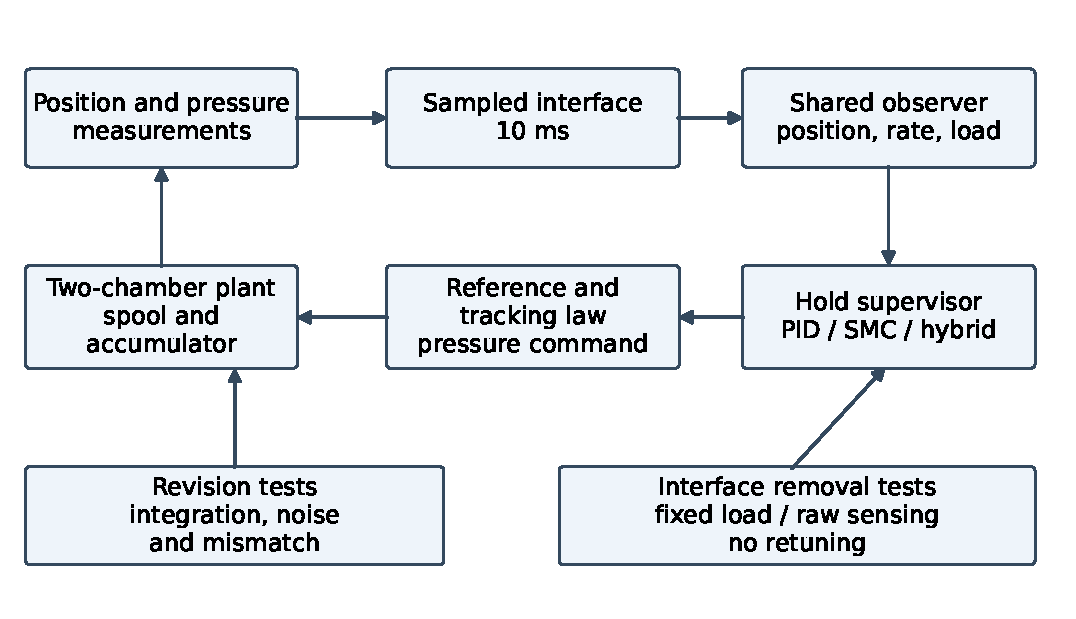
\includegraphics[width=\linewidth]{revision_architecture.pdf}
\caption{Implemented
 feedback and audit interfaces. The~primary four chains share filtered observer outputs. Separate audit arms remove load adaptation or replace the observer by a raw interface; no controller receives true plant velocity or~load.}\label{fig:architecture}
\end{figure}
\unskip

\subsection{Mode-Wise Boundedness and Its~Limits}
The first result concerns the sequential projected numerical model. All pressure states lie in $[p_t,p_{rel}]$, $x\in[0,L]$, the~spool lies in $[-1,1]$ for integration step $h\le0.05$ s, and~accumulator volume lies between its initial gas volume and shell volume. Consequently, accumulator pressure is finite. Let $|F_L|\le\bar F$, $|F_d|\le\bar F_d$ and $B=A(p_{rel}-p_t)+\bar F+kL+\bar F_d$. Here, $F_d$ excludes viscous damping and $\bar F_d=F_c+F_s$ for the implemented dry-friction law: 1200 N nominally and 1560 N for the linked 1.3$\times$ friction arm. The~bound must use each perturbed plant's coefficients. Before~a stroke reset, the~sequential velocity update satisfies Equation~\eqref{eq:discrete-bound}
\begin{equation}
|v_{n+1}|\le\rho|v_n|+hB/m,\qquad \rho=|1-hc/m|<1\quad(0<h<2m/c).
\label{eq:discrete-bound}
\end{equation}

A stroke reset reduces $|v|$ to zero. Iteration gives $|v_n|\le\rho^n|v_0|+hB/[m(1-\rho)]$. This establishes bounded numerical plant states under bounded load for each mode and arbitrary switching. It relies on explicit pressure/stroke projections and is too loose to establish the 10 mm accuracy screen, absence of relief, physical safety, or~convergence. Gaussian measurement noise has no deterministic finite amplitude bound; clipped controls still satisfy this numerical plant-state bound, but~no deterministic observer-accuracy bound is~asserted.

A complementary local argument removes the numerical projections and freezes volumes at a declared operating position $\bar x$. Put $H=1/V_A(\bar x)+1/V_B(\bar x)$ and $d=p_A-p_B$. The~mechanical-pressure subsystem for $y=(x-x_r,v,d)^T$ has the form $\dot y=My+w$, with $M$ defined in Equation~\eqref{eq:local-matrix}:
\begin{equation}
M=\begin{bmatrix}0&1&0\\-k/m&-c/m&A/m\\0&-\beta_e HA&-\beta_e HC_l\end{bmatrix}.
\label{eq:local-matrix}
\end{equation}

The bounded forcing $w$ contains load/reference terms, bounded dry friction, and, in~FINE\_TRIM, spool/accumulator flows. For~a closed, settled spool in LOCK, these flow terms vanish. With~$\ell=\beta_e HC_l>0$ and $K_h=\beta_e HA^2$, the~characteristic polynomial multiplied by $m$ is $m\lambda^3+(m\ell+c)\lambda^2+(c\ell+k+K_h)\lambda+k\ell$. Its coefficients are positive and $(m\ell+c)(c\ell+k+K_h)>mk\ell$; the Routh criterion makes $M$ Hurwitz. Thus, $P>0$ solving $M^TP+PM=-I$ gives Equation~\eqref{eq:local-bound}
\begin{equation}
\dot V\le-\tfrac12\|y\|^2+2\|P\|^2\|w\|^2,\qquad V=y^TPy.
\label{eq:local-bound}
\end{equation}

This is a bounded-input result for a frozen-volume approximation in either mode. The~strict Routh inequality holds for every fixed positive $m,c,k,\beta_e,H,C_l$ and $A$, including the positive parameter perturbations tested here; its Lyapunov matrix depends on the frozen coefficients. This pointwise property does not supply a common matrix for time-varying volumes, parameter changes or switching. In~FINE\_TRIM, the saturated orifice flows are bounded when pressure remains in a specified physical interval, even though they depend on feedback. Volume variation contributes additional terms and must remain a bounded perturbation in a local operating neighborhood. The~argument does not prove that the unprojected nonlinear system stays in that neighborhood. LOCK is not assumed to have a zero-error equilibrium under sustained internal leakage. No global nonlinear or switched-system stability, common Lyapunov function, or~precise holding guarantee follows from the 8 s dwell rule~\cite{liberzon1999,hespanha1999,goebel2009}. The~sequential recurrence above is not used as a discrete proof for RK4; RK4 behavior is evaluated separately by~refinement.

\subsection{Legacy Loss Operator and Corrected Dimensional~Interpretation}
The original manuscript also described a historical pressure-difference surrogate. Its exact loss term is $\mathcal L=\kappa[1+g_T\max(T-25,0)]\max(d,0)/A$ in $\dot d=a_m(d^\star-d)-g_m\mathcal L+(\beta_e/V)q_{acc}$. The~numerical parameter formerly labeled $C_l$ has units m$^2$ s$^{-1}$ in this equation, not m$^3$ s$^{-1}$ Pa$^{-1}$. Writing $\kappa$ makes $\mathcal L$ a pressure rate (Pa s$^{-1}$). This is a correction of the model interpretation, not a physically valid hydraulic leakage law. V2 uses the dimensionally consistent flow law in Equation~\eqref{eq:continuity}.

\textls[-15]{When accumulator flow is zero, pressure is not projected and $g_md_k>0$, inversion gives Equation~\eqref{eq:legacy-proxy}}
\begin{equation}
\kappa_k^*=\frac{A\max[a_m(d_k^\star-d_k)-(d_{k+1}-d_k)/h,0]}{g_md_k[1+g_T\max(T_k-25,0)]},\qquad [\kappa_k^*]=\mathrm{m^2\,s^{-1}}.
\label{eq:legacy-proxy}
\end{equation}

For $\hat\kappa_{k+1}=(1-\alpha)\hat\kappa_k+\alpha\kappa_k^*$ with $0<\alpha\le1$ (historical smoothing $\alpha=0.08$), let $\widetilde\kappa_k=\hat\kappa_k-\kappa_k$. Bounded inversion error $|\kappa_k^*-\kappa_k|\le\bar\epsilon$ and coefficient increment $|\kappa_{k+1}-\kappa_k|\le\nu h$ yield Equation~\eqref{eq:time-varying}
\begin{equation}
|\widetilde\kappa_{k+1}|\le(1-\alpha)|\widetilde\kappa_k|+\alpha\bar\epsilon+\nu h,
\quad \limsup|\widetilde\kappa_k|\le\bar\epsilon+\nu h/\alpha.
\label{eq:time-varying}
\end{equation}

The constant-coefficient case has $\nu=0$; a jump invalidates a rate bound at that step and creates a new transient. Old numerical outputs and their original identifiers remain frozen for traceability, but~physical leakage-identification and flow-unit interpretations are withdrawn. Historical stress and measurement-interface results are summarized in Supplementary S1

, separate from primary V2~evidence.

\subsection{Frozen Evaluation and Additional~Tests}
\label{sec3.6}

\subsubsection{Inputs and Metric Definitions}

The reference is $x_r(t)=0.15+0.20(3\tau^2-2\tau^3)$ m, where $\tau=\min\{t/8,1\}$ for $t\ge0$; its analytic derivatives supply velocity and acceleration feedforward until the reference settles. For~a path with $N$ controller intervals, temperature at sample \mbox{$k$ is $T_k=25+25k/(N-1)$ $^\circ$C}. A~300 s development path therefore traverses the same temperature endpoints faster than an 1800 s test. Development is a separate design task, not a shortened copy of the full-horizon thermal trajectory. The~30 s known-failure diagnostics alone preserve the \mbox{1800 s} ramp~slope.

The original V2 protocol uses 1800 s, a~smooth 0.15 to 0.35 m reference over 8 s, a~9 to 14 kN load step at 60 s, and~a 25 to 50 $^\circ$C temperature ramp. Seeds 4120--4139 form the original test set; seeds 4200--4219 form the existing independent audit. Pass requires hold entry, a hold drop of at most 10 mm, maximum absolute error on the post-transition screen of at most 10 mm, and~zero relief activation. On~the controller grid $t_k=kh_c$, the~entry counter requires 100 consecutive qualifying samples with $t_k\geq8$ s, $|e_k|\leq10$ mm and $|\hat v_k|\leq3$ mm s$^{-1}$. Let $k_c$ be the sample at which the counter reaches 100 and the supervisor enters holding. The~first position included in the implemented drop statistic is the ensuing plant endpoint, $t_h=t_{k_c}+h_c$. For~the recorded endpoint set $\mathcal H=\{k+1:k\geq k_c\}$, the hold drop is $\Delta_h=\max\{0,x_{k_c+1}-\min_{j\in\mathcal H}x_j\}$. This is a sampled statistic, not a continuous-time extremum. The~current output records both the confirmation time $t_{k_c}$ and $t_h$; the earlier timestamp $t_{k_c}-1$ s is retained only in a legacy metadata field and was not the numerical drop window. This timestamp correction changes no historical drop, error, control command or trajectory. Noisy measurements drive the entry gate and controller; reported errors use simulated plant position. The~post-transition screen contains endpoints of controller intervals starting at $t_k\geq8$ s, so its first endpoint is 8.01 s. The~1800 s simulation therefore includes less than 1800 s of confirmed holding. New tests also require zero stroke-boundary~samples.

Let $\mathcal E=\{k:8\le t_k<1800\}$ and $\varepsilon_k=x_r(t_k)-x(t_{k+1})$. The~tabulated tracking metrics are $E_{\max}=\max_{k\in\mathcal E}|\varepsilon_k|$ and $E_{\mathrm{RMS}}=(|\mathcal E|^{-1}\sum_{k\in\mathcal E}\varepsilon_k^2)^{1/2}$. For~development or short diagnostics, the~upper endpoint is the declared path duration instead of 1800 s. On~this interval, $x_r=0.35$ m, so the start-reference/end-state convention introduces no reference-time mismatch. Accumulator oil use is the initial minus final stored-oil volume, clipped below at zero; there is no recharge. If~hold entry is absent, drop is undefined and the path fails; its post-transition errors remain reported. Every fresh-design mean includes all 24 paths, including any failed path with a defined metric. A~zero relief count means that no endpoint pressure proposal exceeded the numerical cap; it does not validate a physical relief~valve.

\subsubsection{Implementation Sequence and Controlled Comparisons}

The additional-audit protocol is fixed in its machine-readable ledger before execution. Observer-interface comparisons use seeds 4300--4309; all sensitivity families use 4300--4304 and preserve the original controller. One arm fixes the load estimate at 9 kN while retaining filters; a second uses raw position, finite-difference velocity and raw pressures with that fixed load. These are interface-removal controls, not an optimally retuned alternative observer. They cross both hybrid and PID--accumulator supervision. Dwell sensitivity uses 0, 2, 4, 8, 12 and 16 s. A~separate PID--accumulator arm applies an 8 s mode latch and gates discharge by its latched support mode; this is a matched-timer diagnostic and changes that baseline's continuous actuation semantics explicitly. An~additional frozen five-seed replay checks each of the other three chains at 1 ms plant~integration.

Mechanical stress changes mass, damping, or~stiffness to 0.7 and 1.3 times nominal, one at a time, while leaving the observer/control coefficients nominal. A~separate predeclared friction-mismatch arm uses the repeated-load schedule and fivefold virtual leakage while scaling the true-plant viscous, Coulomb and Stribeck friction terms together to 0.7 or \mbox{1.3 times} nominal; the observer retains its nominal coefficients. Pressure-noise SD is increased from 0.05 to 0.10, 0.20, 0.50 and 1.00 MPa without external prefiltering. The~original internal observer filter remains active. A~separate joint-noise arm doubles both position and pressure noise. These distinctions prevent a pressure-only test from being confused with the original doubled-all-sensors~test.

Integration refinement keeps controller sampling at 10 ms, freezes every measurement-noise sample and commanded input over that interval, and~splits only the plant update into $h=10,5,2.5,1$ ms. The~submitted 10 ms path is an explicit sequential update. After~one observer/controller update, each plant substep updates the spool, computes chamber flows and pressure increments, and~projects the new pressures into their declared interval. Mechanical acceleration then uses these updated pressures and the previous velocity in the friction law; velocity is advanced, position uses the updated velocity, stroke crossings reset velocity, and~accumulator gas volume advances using that substep's discharge. This plant ordering is repeated at each substep, without~additional observer/controller updates. The~10 ms choice supplies five controller samples per 50 ms spool time constant but is not an a priori accuracy guarantee for chamber pressure. This isolates solver sensitivity from a changed noise bandwidth or observer discretization. The~discontinuous friction and projection rules are unchanged. We therefore report sampled pressure-path discrepancies against 1 ms in addition to holding metrics. Seed 4300 is the predeclared representative trajectory; the code supplies its position, pressures, accumulator state and modes. Reported confidence intervals describe seeded model noise, not a physical-machine~population.

As a higher-order numerical audit, the~same five seeds were replayed with a classical fourth-order Runge--Kutta update for the virtual plant at 1.0 and 0.5 ms steps. Controller updates, observer updates, measurement draws, commands and mode decisions remained on the original 10 ms grid. Pressure and stroke crossings were projected at the end of each plant step and the velocity was reset at a stroke event. No gains or thresholds were retuned. This arm tests fine-step numerical convergence; it does not replace the frozen original Euler protocol or add a physical-model~claim.

For RK4, the~joint state is $y=(x,v,p_A,p_B,z,V_g)$ and the six simultaneous rates are evaluated at the four classical stages. With~step $h$, $K_1=f(y_n)$, $K_2=f(y_n+hK_1/2)$, $K_3=f(y_n+hK_2/2)$ and $K_4=f(y_n+hK_3)$; the proposal is $y_{n+1}^{\star}=y_n+h(K_1+2K_2+2K_3+K_4)/6$. Measured inputs, controller commands, load and temperature remain fixed within a controller interval. Flow and friction rates use each stage state; pressure/stroke/spool/storage projections are applied to the completed proposal. This differs from the sequential explicit update above and is why the solver arms are labeled separately. No event-root solver or physical impact law is~introduced.

The paired RK4 comparison also includes the original PID--accumulator and its separate 8 s latch/discharge-gating diagnostic at both plant steps, using seeds 4300--4304, unchanged sensing and frozen gains. Ten existing hybrid runs are reused with source hashes; the two PID arms add 20 runs. A~separate predeclared joint screen evaluates all eight vertices of $(m/m_0,c/c_0,k/k_0)\in\{0.7,1.3\}^3$ with the hybrid, five common seeds per vertex, a~1 ms RK4 plant step and nominal controller/observer coefficients. Each true plant starts from its own declared force-balance initial pressure; all paths retain the same reference, load step and temperature ramp. The~40 joint runs are reported in full. This finite corner screen neither samples the full box interior nor certifies robust invariance. The~two RK4 steps use endpoint projections without event-root localization, so classical fourth-order convergence is not asserted for friction or projection~events.

For the combined-stress audit, a~separate protocol was declared before execution. It repeats the load schedule $(0,9),(60,14),(300,10),(600,16),(900,11),(1200,15)$ kN, uses the 1800 s reference and 10 ms controller period, and~evaluates seeds 4400--4404. The~nominal arm uses the declared leakage coefficient; the sustained-leakage arm multiplies that coefficient by five; and the ablation arm uses the same fivefold leakage and sets the accumulator valve command to zero. The~ablation changes one actuator path only; it does not retune the observer, thresholds or tracking gains. The~machine-readable protocol and all 15 traces are supplied in the reproduction code/results ZIP, separately from the manuscript-source ZIP. The~friction-mismatch extension uses the same seeds and combined schedule; no gain, threshold, observer or controller coefficient is~retuned.

\subsubsection{Additional Independent Risk-Closure Protocol}
The frozen submitted gains remain distinct from a new equal-budget development comparison. Each policy receives nine candidates. Tracking multipliers are $g_t\in\{0.7,1,1.3\}$; accumulator multipliers are $g_a\in\{0.5,1,1.5\}$. The~multiplier $g_t$ scales the 650 and 90 feedback gains and the PID integral gain 20, but~leaves reference feedforward unchanged; $g_a$ scales the complete accumulator command before saturation. Both policies use the same $\pm0.10$ main-valve authority, 8 s dwell and mode-gated discharge. Mode-request thresholds remain policy-specific. Thus, authority, timing and search effort are matched without making the policies identical. Three development seeds (4600--4602), 300 s paths and 1 ms RK4 are used per candidate. The~development load schedule is $(0,9),(60,14),(100,10),(160,16),(220,11),(260,15)$ kN with fivefold leakage. Candidates are ranked by failure count, then mean $J=\Delta_h/10+\mathrm{RMSE}/10+V_{acc}/500+N_{sw}/225$, using mm and mL. These fixed engineering normalizations express one preference, not universal utility weights. All candidates and their four-objective nondominated subset are retained. Selection is recorded before the independent 1800 s evaluation on seeds 4700--4709, using the full repeated-load schedule at both 1 and 0.5 ms. No validation outcome changes selection. Both policies share each seed's measurement sequence and initial plant state. This finite grid is not a global optimization or a comparison against all robust-control~methods.

A separate convergence screen repeats nominal leakage, fivefold leakage, accumulator-disabled and linked $0.7/1.3\times$ friction arms at 1 and 0.5 ms on seeds 4400--4402, without~retuning the submitted controller. A~24-path stratified interior screen uses new seeds \mbox{4800--4823} and independently permuted bins for 12 simultaneous inputs: mass, viscous damping, stiffness, Coulomb friction, Stribeck amplitude and velocity scale, bulk modulus, spool lag, leakage multiplier, accumulator flow coefficient, pressure-noise amplitude and position bias. The~intervals and all sampled inputs are supplied in Supplementary S10. These are virtual-design intervals, not calibrated distributions. The~controller retains the original gains and nominal force-balance coefficients. It contains no explicit Coulomb/Stribeck compensation; these unmodeled terms can enter its effective-load estimate. Independent friction magnitudes and velocity scales test more than a linked scaling, but~the functional friction law itself remains~fixed.


\subsubsection{Active Nonlinear Comparison and Verified Execution}
The active sliding-mode (SMC) chain uses $1200\tanh[(18e+e_v)/0.006]$ N with the common observer, pressure PI, nominal force-balance coefficients and $\pm0.10$ holding authority, without~the PID position integral. The~main valve remains active during holding. The~support threshold is $e>2$ mm. Its accumulator command is
\[
u_{acc}=\operatorname{clip}_{[0,1]}[80g_a\max(e-0.001,0)].
\]

Discharge additionally requires the latched ACCUMULATOR label. Both active baselines explicitly receive the same 8 s latch argument; their initial FINE\_TRIM label is retained until the latch expires. The~hybrid has its stated policy-specific hysteresis and the same 8 s minimum dwell. The~control interfaces and budgets are matched, while the decision rules remain different. This is an executable boundary-layer comparator informed by the sliding-mode family~\cite{tang2011,guan2008}; it does not reproduce a published adaptive design or prove reaching of the full saturated~loop.

A final execution audit found that an earlier SMC runner supplied zero rather than 8 s to the latch argument, also bypassing mode-gated discharge. Its records remain archived as an unlatched diagnostic and are excluded from matched-baseline claims. A~separately frozen correction repeats all nine SMC candidates on the same development seeds \mbox{4600--4602}, 300 s schedule, 1 ms RK4 and unchanged scalar objective. Selection uses only those corrected development outcomes. Corrected SMC replays of common nominal seeds 4700--4709 at 1 and 0.5 ms, known vectors 4800--4823 and previously examined vectors 4900--4923 are follow-up checks, not fresh holdouts. Changes relative to the unlatched arm combine execution correction with reselection; they do not isolate a causal effect of dwell~alone.

\subsubsection{Separate Accuracy Preference and New Joint Verification}
The scalar-selected hybrid and PID remain frozen at $(g_t,g_a)=(1,0.5)$ and $(1.3,0.5)$. The~margin hybrid remains the original development-grid choice $(1.3,0.5)$: require no development failure and worst development error $\le8$ mm, then minimize the same $J$ and candidate ID. Its 2 mm reserve is a heuristic for the stated bias amplitude, not a total observer-error bound. No result from a joint design changes these choices. Corrected SMC selection applies the same nine-candidate rule, and~its eligibility under the 8 mm constraint is reported separately. Development-only weight profiles remain sensitivity checks rather than test-based~tuning.

Before corrected development, random seed 51191 freezes 24 new stratified vectors over the same twelve intervals, with~noise seeds 5100--5123. All four policy instances face identical true-plant overrides, measurement-noise sequences, reference, repeated-load schedule, initial state and 1 ms RK4 integration. The~measured values themselves differ with each policy's plant trajectory. These are the new joint verification outcomes; the earlier 4900-series outcomes are identified as previous-design follow-up. The~new correction contains 27 development paths and 164 full-horizon paths: 68 corrected SMC follow-ups and 96 new four-policy joint paths. Selection files, actual execution arguments, sampled inputs and every failed path accompany the checkpoints. The~intervals are numerical design choices without physical-frequency~interpretation.


\subsection{Supply Availability and Conditional Storage~Support}\label{sec:supply-method}
The continuously available supply in the preceding experiments can conceal a storage contribution: active trim can replace lost fluid. A~separate experiment therefore tests a declared supply-availability boundary. Let $\chi_k\in\{0,1\}$ indicate the availability of the supply-connected main-valve orifice during controller interval $k$. With~$Q$ defined \mbox{in Section~\ref{sec3.1}}, the~additional flow law is Equation~\eqref{eq:supply-flow}
\begin{equation}
 (q_A,q_B)=
 \begin{cases}
 (\chi_k Q(a,p_s-p_A),\ Q(a,p_B-p_t)),&z\ge0,\\
 (-Q(a,p_A-p_t),\ -\chi_k Q(a,p_s-p_B)),&z<0.
 \end{cases}\label{eq:supply-flow}
\end{equation}

Thus, $\chi=0$ disconnects supply while retaining the return-connected orifice. Every policy has the same valve, finite accumulator, spool lag, return path and availability signal; electronic control and sensing remain powered. Existing policies retain their original decision rules, while the extension explicitly conditions storage allocation on $\chi$. The~initial states and all other plant equations are unchanged. The~signal is an ideal test input with no detection delay or uncertainty; it is not a pressure-collapse, hose-break, cavitation, or~fault-diagnosis model. Its future switching times do not enter a controller decision. Figure~\ref{fig:physical-system} depicts the normal circuit abstraction; Equation~\eqref{eq:supply-flow} specifies this additional~intervention.

\subsubsection{A Necessary Balance for Stationary Holding}
Within the unprojected model, fix a nonzero supported load and suppose that $v=\dot p_A=\dot p_B=0$, with~$\chi=0$ and $z\ge0$. The~two chamber continuity equations require the balance in Equation~\eqref{eq:reserve-balance}
\begin{equation}
 q_{acc}=q_l=q_B,
 \qquad q_l=C_l\theta_T(p_A-p_B)>0.\label{eq:reserve-balance}
\end{equation}

Here, $\theta_T$ is the stated temperature factor. A~storage inflow and a return outflow are both necessary for this stationary piston/chamber balance. Gas volume continues to increase, so this is not a steady state of the complete finite-storage system. Blocking both main ports instead imposes $q_B=0$, which is incompatible with positive leakage and the assumed nonzero pressure difference. Feeding only chamber A cannot sustain that chamber balance: pressure builds in chamber B until available discharge head decreases. This is a continuity argument under the stated conditions; compliance can permit a storage-disabled path to satisfy a finite displacement tolerance~temporarily.

Finite storage further requires $p_g>p_A$ while discharging. Writing $p_g=K_g V_g^{-n}$, the~volume deliverable before a fixed required head $p_{req}$ is reached is at most the bound in Equation~\eqref{eq:reserve-head}:
\begin{equation}
 \Delta V_{head}=\max\!\left[0,\min\!\left(V_{shell},
 (K_g/p_{req})^{1/n}\right)-V_{g,0}\right].\label{eq:reserve-head}
\end{equation}

Here, $V_{g,0}$ denotes gas volume at the start of the interval being considered. The~expression assumes a fixed positive required head and ignores flow restrictions; it is an optimistic volume bound, not a certified holding duration. Return throttling, changing load, sensing error and pressure projections prevent interpreting it as a closed-loop~guarantee.

\subsubsection{Availability-Aware Hybrid Probe}
The additional policy uses the scalar hybrid's force/pressure and ordinary actuation branches when $\chi=1$, with~its previously selected $(g_t,g_a)=(1,0.5)$. On~an always-available path, it is identical to that hybrid. Once holding has been confirmed and $\chi=0$, it retains the same nominal force-balance target and pressure PI. The~main command becomes $u=\operatorname{clip}_{[0,0.10]}(u_{PI})$, permitting B-to-tank return without an available A supply. Define $d=\Delta p^*-\widehat{\Delta p}$. An~8 s dwell latch requests RESERVE when $d>0.03$ MPa or $e>1$ mm, and~requests ISOLATED when $d<0.01$ MPa and $e<0.5$ mm. While latched in RESERVE, the command follows Equation~\eqref{eq:reserve-control}:
\begin{equation}
 u_{acc}=\operatorname{clip}_{[0,1]}\!\left\{
 g_a\left[1.5\frac{\max(d-0.02\,{\rm MPa},0)}{1\,{\rm MPa}}
       +60\,{\rm m}^{-1}\max(e-0.5\,{\rm mm},0)\right]\right\};\label{eq:reserve-control}
\end{equation}
otherwise, $u_{acc}=0$. Restoration of $\chi=1$ resets the reserve latch and resumes the original hybrid decision branch. The~ordinary mode history and timer remain in force; a retained RESERVE or ISOLATED label receives bounded trim and zero storage command until an ordinary transition becomes eligible. A~supply event can change the policy label independently of the ordinary mode timer. The~hold latch remains one-way. The~probe jointly changes the interruption command sign constraint and support thresholds; the comparison does not isolate the value of availability information alone. It adds an engineering allocation rule, without~a new observer or a nonlinear stability theorem, and~is distinct from the earlier 8 mm development-margin~hybrid.

\subsubsection{Fixed Experiment and Resource Accounting}
Exploratory seeds 5200--5202 include both-port blocking and supply-only disconnection; all their failures remain archived. They are excluded from the prospective verification. The~earlier hybrid/PID/corrected-SMC gain choices remain $(1,0.5)$, $(1.3,0.5)$ and $(1.3,0.5)$; no resource objective or new validation outcome reselects them. Thus, the resource comparison concerns these frozen instances, not policies optimized for input work. Each uses the same $\pm0.10$ holding authority, common measurements and 10 ms controller period. PID and SMC both receive their explicit 8 s latch/discharge~gate.

Before execution, a~separate protocol fixes 88 paths of 1800 s: four new normal-supply repeated-load seeds under each of four policies (16 paths); eight new stratified joint parameter/sensing vectors, supply disconnected on $[300,1500)$ s, with~storage enabled and disabled under each policy (64 paths); and the predeclared first joint vector repeated at \mbox{0.5 ms} for both storage states under all policies (eight paths). Other paths use 1 ms coupled RK4. The~interruption family has the original 60 s load step followed by its sampled constant load; it is distinct from the repeated-load normal family. Supplementary S12 gives all \mbox{13 sampled} intervals, vectors, failures, and~paired differences. The~eight-vector design is small and has no physical-frequency~interpretation.

Four-stage RK4 quadrature records the actual positive supply-orifice flow $q_s=q_A$ for $z\ge0$ and $q_s=-q_B$ for $z<0$. Over~the same controller intervals starting at 8 s (endpoints 8.01--1800 s), report the quantities in Equation~\eqref{eq:boundary-resource}:
\begin{equation}
 V_s=\int q_s\,dt,\qquad
 W_g=\int p_gq_{acc}\,dt,\qquad
 B=p_sV_s+W_g.\label{eq:boundary-resource}
\end{equation}

These quantities use a common window rather than policy-dependent hold-entry times. $B$ is a boundary-resource index for the declared constant-pressure source and storage outlet. It excludes pump efficiency, standby power, line dynamics, recharge and the energy effects of numerical projections. Consequently, neither $B$ nor its percentage difference is a measured system-energy saving. Storage remains initially charged and is not recharged during a path. Mode counts with different policy labels are not interpreted as comparable mechanical~wear.


\subsubsection{Separate Resource-Oriented Gain Selection}
The normal-supply comparison is additionally challenged by a new resource-oriented search, declared after the earlier results but before its own outcomes. Each of scalar hybrid and active SMC receives the same nine $(g_t,g_a)$ candidates, $\{0.7,1.0,1.3\}\times\{0.3,0.5,0.7\}$, and~three new development seeds, 5600--5602. All 54 development paths use the complete 1800 s repeated-load schedule, fivefold leakage and 1 ms RK4. Holding authority, sensing, observer, 8 s latch and discharge gate are shared. Candidates are ranked lexicographically by number of failed development paths, mean $B$ in Equation~\eqref{eq:boundary-resource}, and~candidate ID. The~feasibility screen requires confirmed hold, both 10 mm limits and no relief or stroke event. A~zero-failure candidate is development-feasible; if none exists, the least-failing candidate remains explicitly infeasible. Selection is frozen before eight additional 1800 s validation paths: seeds 5620--5623 under each selected policy. Every candidate and outcome is retained in Supplementary S13. This is a bounded gain search, not a global resource frontier: SMC's 1200 N boundary-layer amplitude and 0.006 m/s width, hybrid thresholds and other architecture constants remain fixed. Validation concerns normal supply and the nominal plant with the specified leakage; it supplies no new joint-uncertainty or interruption~guarantee.


\section{Results}
The controller-version summary at the end of this section

lists the controller versions, selection objectives, adopted gains, integration steps and seed roles in Sections~\ref{sec4.1} and \ref{sec4.8}--\ref{sec:resource-retuning}. The~result families answer different questions. Sections~\ref{sec4.1}--\ref{sec4.7} retain the submitted-gain comparison, component removals and specified perturbations. Section~\ref{sec4.8} tests a separately selected hybrid/PID pair with a common development budget. Section~\ref{sec4.9} distinguishes previously examined joint vectors from a newly frozen joint design and uses an explicitly matched active nonlinear baseline. Gains, gates and seed roles are identified for each family; a favorable result from one version is not substituted for another version's~failure.

\subsection{Frozen Comparison with Uncertainty~Estimates}
\label{sec4.1}

The primary comparison remains the original 20-seed set 4120--4139. Table~\ref{tab:comparison} adds seed-to-seed sample standard deviations and confidence intervals without changing its trajectories. Both active holding chains passed 20/20, while PID--lock and \mbox{sliding-mode--lock} failed after the load step. The~hybrid's mean and worst hold drops were 1.85 and \mbox{2.10 mm}; the worst post-transition error was 8.90 mm. PID--accumulator achieved a smaller post-transition RMSE (0.25 versus 1.22 mm), but~a larger mean hold drop (3.44 mm). No path activated pressure relief. The~comparisons support a model-specific tracking--holding trade-off.





Figure~\ref{fig:comparison} displays the frozen comparison and its between-seed variability.
\begin{figure}[H]
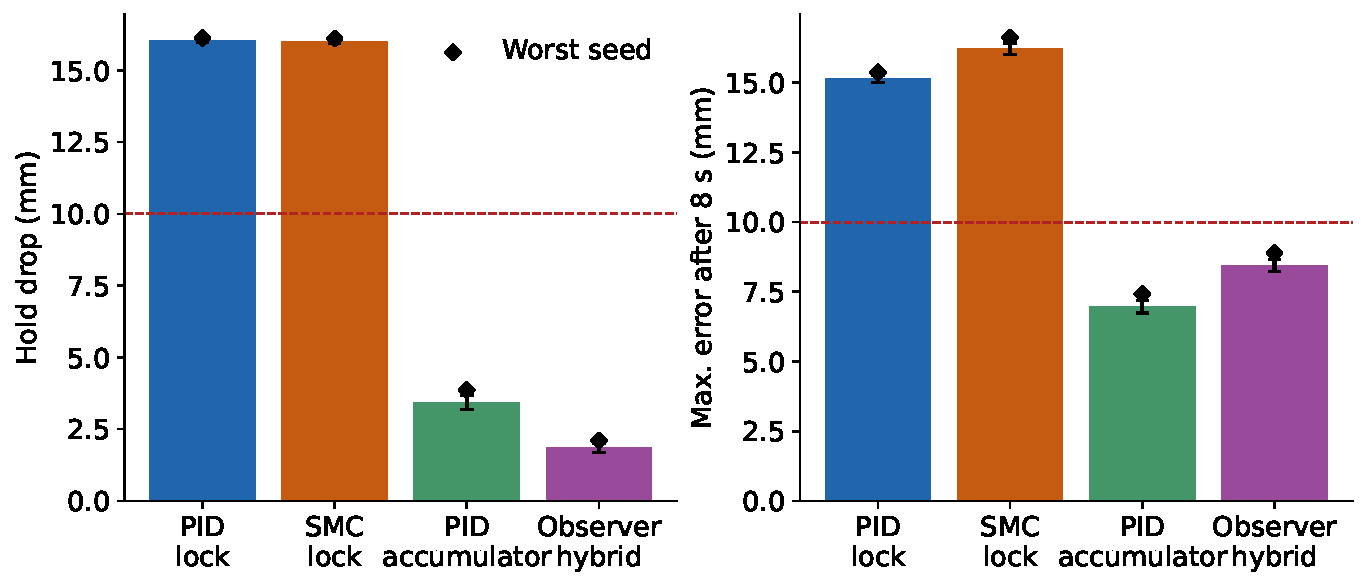
\includegraphics[width=\linewidth]{revision_comparison.pdf}
\caption{Frozen
 V2 results with sample SD error bars and worst-seed diamonds, $n=20$. The~dashed line is the 10 mm screen. Mean error bars do not imply that every trajectory~passes.}\label{fig:comparison}
\end{figure}

The existing independent audit on seeds 4200--4219 passed 20/20 with a mean hold drop of 1.89 mm and worst drop of 2.12 mm. The~independent fivefold-leakage, doubled-noise and half-flow groups also passed 10/10 each. These sets remain independent of tuning. Confidence intervals quantify the stated seeded-noise process in one virtual plant, not uncertainty in the physical parameter~values.


\begin{table}[H]

\caption{Frozen 20-path V2 comparison with between-seed sample SD and two-sided Student-t 95\% interval for mean hold~drop.}\label{tab:comparison}
\small
\begin{tabularx}{\textwidth}{lc CC c}
\toprule
\textbf{Controller} & \textbf{Pass} & \textbf{Drop Mean} \boldmath{$\pm$} \textbf{SD (mm)} & \textbf{Mean-Drop 95\% CI (mm)} & \textbf{Worst Error (mm)} \\
\midrule
PID--lock & 0/20 & 16.04 $\pm$ 0.06 & 16.01--16.07 & 15.38 \\
SMC--lock & 0/20 & 15.99 $\pm$ 0.06 & 15.97--16.02 & 16.62 \\
PID--accumulator & 20/20 & 3.44 $\pm$ 0.25 & 3.32--3.56 & 7.43 \\
Observer hybrid & 20/20 & 1.85 $\pm$ 0.16 & 1.78--1.92 & 8.90 \\
\bottomrule
\end{tabularx}
\end{table}


\vspace{-9pt}

Figure~\ref{fig:load-step} shows the position and chamber-pressure responses of the predeclared representative path.
\begin{figure}[H]
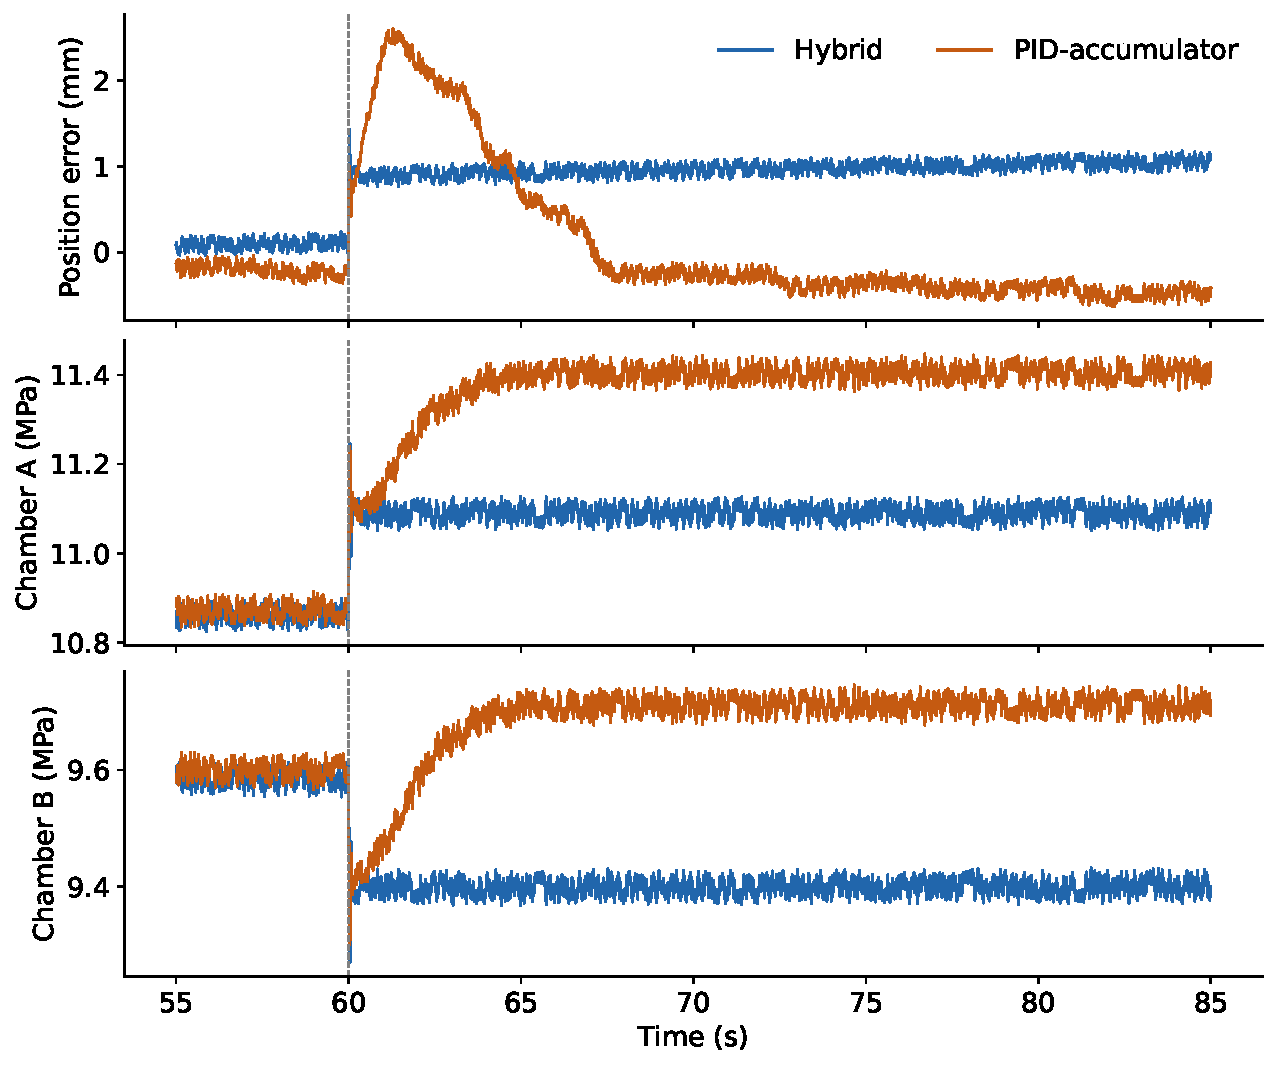
\includegraphics[width=0.95\linewidth]{revision_load_step.pdf}
\caption{Position
 error and separately conserved chamber pressures after the 60 s load step. Seed 4300 was fixed before additional tests; it is not selected for favorable accuracy. Curves use the original 10 ms plant~integration.}\label{fig:load-step}
\end{figure}
\unskip

\subsection{Repeated-Load and Sustained-Leakage~Audit}
The new stress protocol combines repeated load changes with a leakage coefficient five times the declared V2 value. All three arms entered hold on all five seeds, and~all paths passed the 10 mm drop/error and zero-relief screen. With~nominal leakage, the~mean and worst hold drops were 2.56 and 2.81 mm; with fivefold leakage, they were 2.68 and 3.77 mm. The~mean post-transition maximum errors were 8.47 and 8.48 mm, respectively. The~fivefold arm generated more mode changes (55.8 on average) but still did not activate the relief path or reach a stroke boundary. These results show that repeated changes and sustained leakage can be evaluated together without selecting a favorable single~transition.

The accumulator-disabled arm passed the same five paths with a mean hold drop of \mbox{2.68 mm} and worst drop of 3.77 mm, and~its mean post-transition maximum error was \mbox{8.48 mm}. Accumulator oil use was zero by construction. The~enabled nominal and fivefold-leakage arms used 38.13 and 36.02 mL mean oil, respectively; the latter reached a minimum accumulator pressure of 13.59 MPa. Thus, the present schedule does not demonstrate that storage is necessary for this virtual plant. It does demonstrate the requested ablation boundary: the tested holding result is not dependent on an unreported accumulator contribution under these particular load and leakage values. Stronger storage-demanding disturbances and a calibrated recharge model remain outside the current theoretical~scope.

Table~\ref{tab:reviewer3-stress} reports every combined-stress arm.
\begin{table}[H]
\setlength{\tabcolsep}{3pt}
\caption{Predeclared
 repeated-load and sustained-leakage audit, five seeds per arm. The~5$\times$
 leakage factor multiplies the declared internal V2 coefficient; it is a virtual stress input, not a calibrated fault~condition.}\label{tab:reviewer3-stress}
\small

\begin{adjustwidth}{-\extralength}{0cm}

\begin{tabularx}{\fulllength}{l cc cccc}
\toprule
\textbf{Arm} & \textbf{Entry} & \textbf{Pass} & \textbf{Mean Drop (mm)} & \textbf{Worst Drop (mm)} & \textbf{Worst Error (mm)} & \textbf{Mean~Switches} \\
\midrule
Nominal leakage, accumulator enabled & 5/5 & 5/5 & 2.56 & 2.81 & 8.62 & 17.0 \\
5$\times$ leakage, accumulator enabled & 5/5 & 5/5 & 2.68 & 3.77 & 8.63 & 55.8 \\
5$\times$ leakage, accumulator disabled & 5/5 & 5/5 & 2.68 & 3.77 & 8.63 & 55.8 \\
\bottomrule
\end{tabularx}
\end{adjustwidth}
\end{table}
\unskip

Figure~\ref{fig:reviewer3-stress} shows the representative repeated-load trajectory.
\begin{figure}[H]
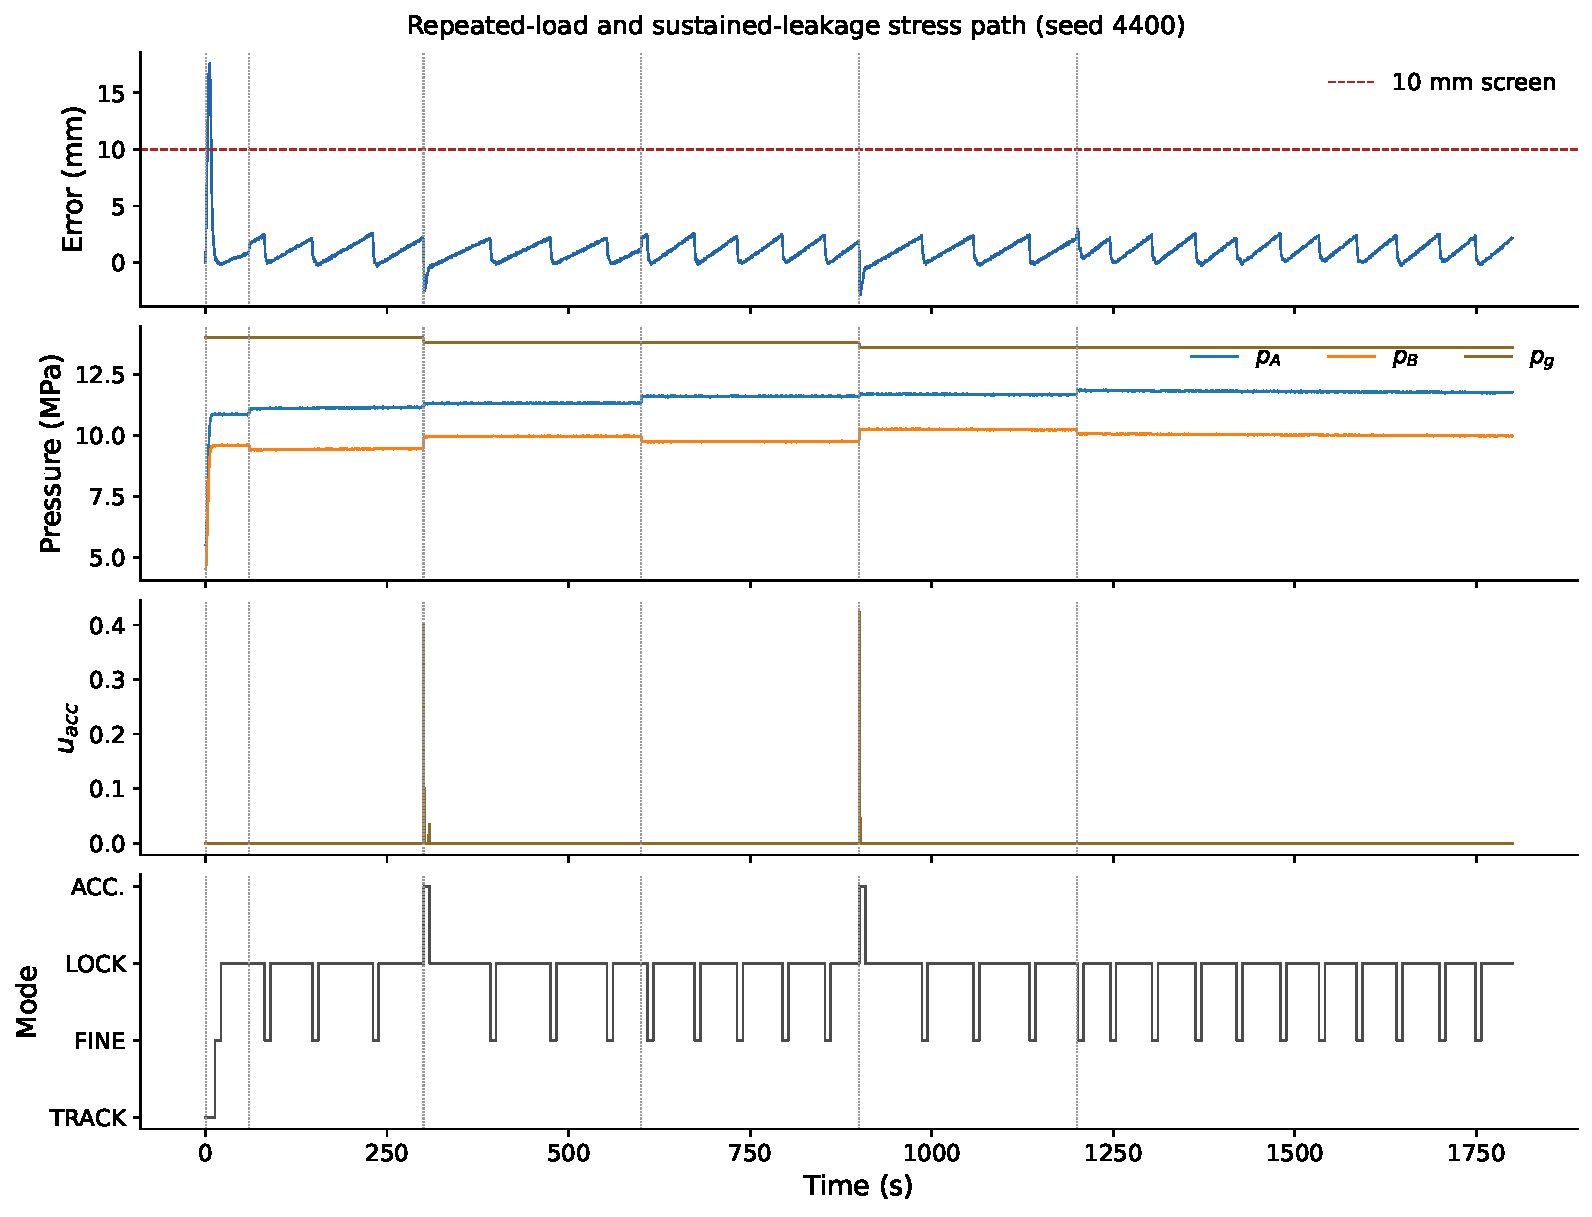
\includegraphics[width=0.98\linewidth]{reviewer3_repeated_load.pdf}
\caption{Representative
 repeated-load and sustained-leakage path (seed 4400). Vertical lines mark the predeclared load changes. The~panels show the simulated position error, chamber and accumulator pressures, accumulator command, and~discrete supervisor~mode.}\label{fig:reviewer3-stress}
\end{figure}
\unskip




\subsection{Observer and Supervisor~Contributions}
The crossed interface-removal tests in Table~\ref{tab:observer} distinguish effects that the shared-observer comparison could not identify. Retaining filtering while fixing the load estimate at 9 kN increased the hybrid's mean drop from 1.94 to 5.87 mm and mean accumulator use from zero to 232.0 mL. All ten paths still passed, so adaptive load estimation is not necessary for passing this particular screen; it materially changes drift and stored-fluid use. PID--accumulator shows a similar oil-use increase. Replacing the entire observer by raw position, finite-difference velocity and raw pressures prevented hold entry in every path of both control chains. The~raw differentiated position noise violates the velocity gate frequently. These removal tests establish dependence on the implemented interface; they do not separate every observer gain or show superiority to a properly designed alternative~observer.

Figure~\ref{fig:reviewer3-ablation} compares storage-enabled and storage-disabled traces under the preceding stress protocol.
\begin{figure}[H]
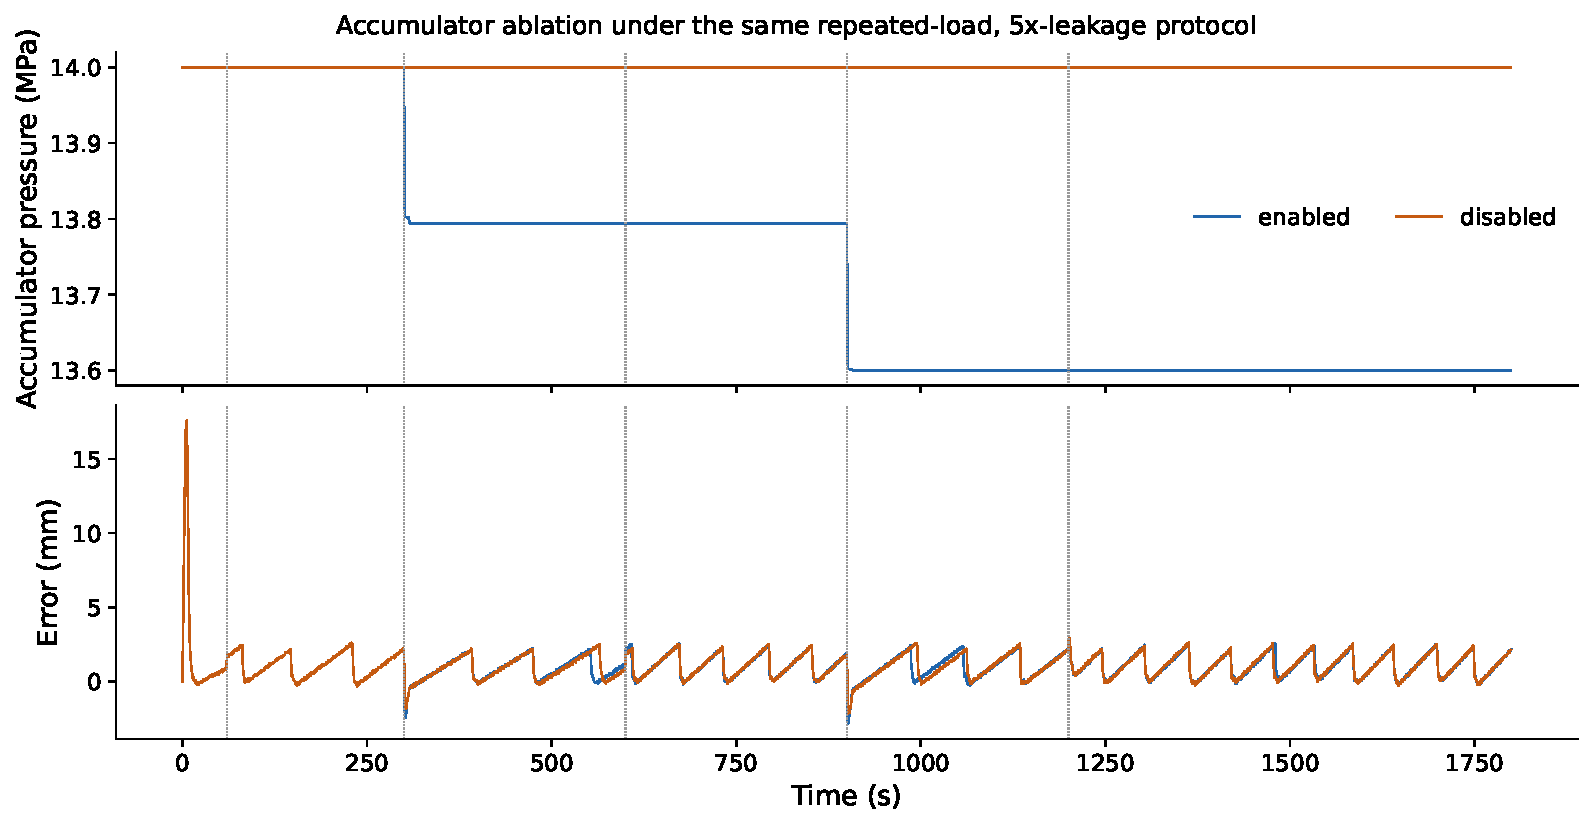
\includegraphics[width=0.98\linewidth]{reviewer3_accumulator_ablation.pdf}
\caption{Accumulator-enabled
 and accumulator-disabled traces under the same repeated-load and fivefold-leakage protocol. The~disabled arm is an actuator ablation, not a retuned~controller.}\label{fig:reviewer3-ablation}
\end{figure}


\vspace{-9pt}

\begin{table}[H]

\caption{Crossed observer-interface removal tests on seeds 4300--4309. A~dash denotes no hold entry; failed paths remain in maximum-error~statistics.}\label{tab:observer}
\small
\begin{tabularx}{\textwidth}{l cc CC C}
\toprule
\textbf{Control and Interface} & \textbf{Entry} & \textbf{Pass} & \textbf{Mean Drop (mm) }& \textbf{Worst Error (mm)} & \textbf{Oil (mL)} \\
\midrule
Hybrid: Shared observer & 10/10 & 10/10 & 1.94 & 8.93 & 0.0 \\
Hybrid: Fixed load & 10/10 & 10/10 & 5.87 & 9.94 & 232.0 \\
Hybrid: Raw interface & 0/10 & 0/10 & -- & 23.11 & 0.0 \\
PID--acc.: Shared observer & 10/10 & 10/10 & 3.51 & 7.45 & 25.3 \\
PID--acc.: Fixed load & 10/10 & 10/10 & 5.94 & 8.47 & 237.8 \\
PID--acc.: Raw interface & 0/10 & 0/10 & -- & 21.59 & 0.0 \\
\bottomrule
\end{tabularx}
\end{table}
\unskip


\subsection{Dwell Sensitivity and a Matched-Timer~Baseline}
All six dwell settings passed the five-path additional screen (Table~\ref{tab:dwell}). Removing the hybrid dwell raised the mean mode-switch count from 13.0 to 58.8, while mean hold drop changed from 1.883 to 1.977 mm. Thus, the timer accounts for a substantial fraction of the observed low switching activity. The~12 and 16 s settings also gave 13.0 mean switches with mean drops near 1.92 mm; the chosen 8 s value is not a unique robust optimum. All 27 original development candidates passed five development paths. The~archived ranking and the post-selection sensitivity ledger expose the search budget and alternative~settings.

\begin{table}[H]

\caption{Frozen hybrid dwell sensitivity, five paths per row. All other thresholds and controller settings remain~unchanged.}\label{tab:dwell}
\small
\begin{tabularx}{\textwidth}{l@{\hspace{3em}} c @{\hspace{3em}}c @{\hspace{3em}}c@{\hspace{3em}} c}
\toprule
\textbf{Dwell (s)} & \textbf{Pass} & \textbf{Switches (Mean)} & \textbf{Mean Drop (mm)} & \textbf{Mean Oil (mL)} \\
\midrule
0 & 5/5 & 58.8 & 1.977 & 1.62 \\
2 & 5/5 & 17.4 & 1.931 & 0.00 \\
4 & 5/5 & 14.6 & 1.924 & 0.00 \\
8 & 5/5 & 13.0 & 1.883 & 0.00 \\
12 & 5/5 & 13.0 & 1.919 & 0.00 \\
16 & 5/5 & 13.0 & 1.916 & 0.00 \\
\bottomrule
\end{tabularx}
\end{table}


In the new matched-timer diagnostic, PID--accumulator with an 8 s latch and discharge gated by its support mode passed 5/5, with~3.0 mean mode changes, 3.475 mm mean hold drop and 23.91 mL mean oil use. The~hybrid on identical seeds had 13.0 changes, \mbox{1.883 mm} drop and zero oil use. Consequently, the original reduction from 26.8 to 13.1 switches cannot be attributed to intrinsically better supervisory logic independent of dwell or actuator gating. The~hybrid retains a smaller drop and less oil use in this comparison, but~does not retain a switching-count advantage. Neither mode labels nor oil volume measure valve wear or total hydraulic~energy.

Figure~\ref{fig:dwell} summarizes dwell sensitivity and the matched-timer diagnostic.
\begin{figure}[H]
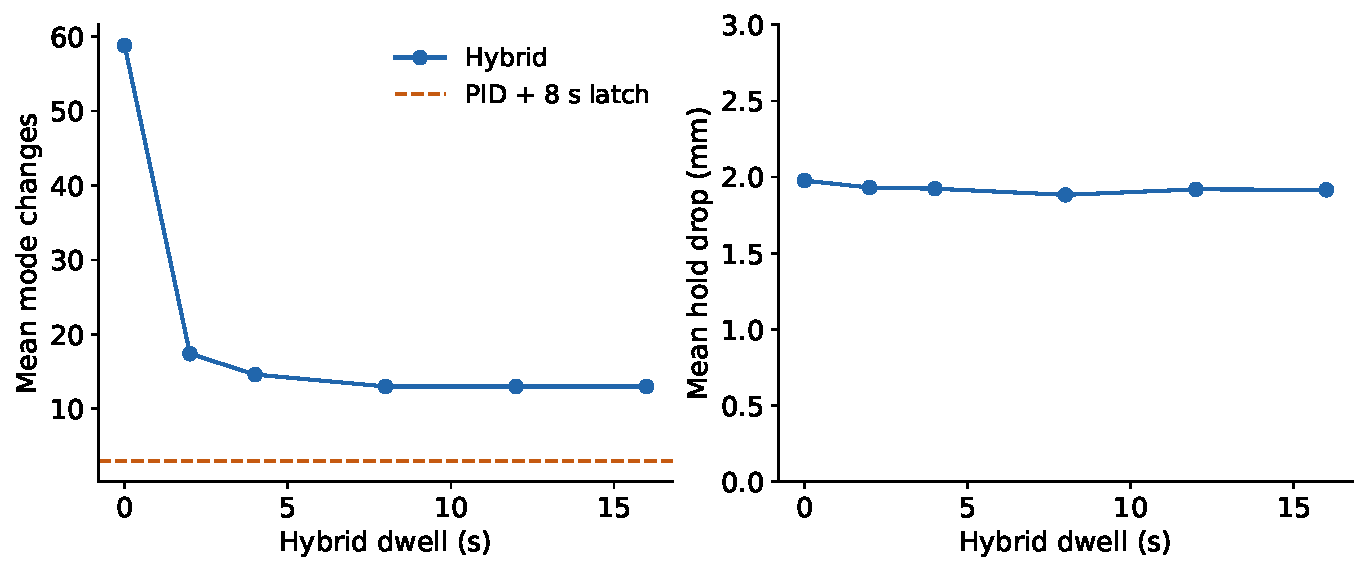
\includegraphics[width=\linewidth]{revision_dwell.pdf}
\caption{Dwell-time
 sensitivity and the separate matched-timer PID diagnostic. The~PID diagnostic changes the original baseline's discharge gating and therefore is not a bitwise replay of that~baseline.}\label{fig:dwell}
\end{figure}
\unskip

\subsection{Integration Refinement and Pressure~Dynamics}
All five hybrid paths passed at 10, 5, 2.5 and 1 ms plant steps under fixed 10 ms sensing and control (Table~\ref{tab:integration}). The~mean hold drop decreased from 1.883 to 1.732 mm; the worst error decreased from 8.927 to 8.765 mm. The~former is about an 8\% change relative to the coarse mean, so the coarse numerical values are not precision-converged. Their pass/fail status and the scale of the holding response are retained on these paths. Pressure discrepancies against the 1 ms replay are reported in Supplementary S4, including full-horizon RMS and maximum sampled differences, rather than hidden behind matching pass rates. Different switching times and discontinuous low-speed friction can make long-horizon maximum differences larger than the local load-step discrepancy. The~study does not establish a formal convergence order for this nonsmooth~integrator.

\begin{table}[H]

\caption{Plant integration refinement at a fixed 10 ms controller and measurement period with identical noise~samples.}\label{tab:integration}
\small
\begin{tabularx}{\textwidth}{l c@{\hspace{2em}}c@{\hspace{2em}}c@{\hspace{2em}}c}
\toprule
\textbf{Plant Step (ms)} & \textbf{Pass} & \textbf{Mean Drop (mm)} & \textbf{Worst Error (mm)} & \textbf{Peak Pressure (MPa)} \\
\midrule
10 & 5/5 & 1.883 & 8.927 & 11.293 \\
5 & 5/5 & 1.862 & 8.845 & 11.247 \\
2.5 & 5/5 & 1.831 & 8.795 & 11.231 \\
1 & 5/5 & 1.732 & 8.765 & 11.222 \\
\bottomrule
\end{tabularx}
\end{table}


The other three frozen chains were also replayed at 1 ms on the same five seeds. PID--lock and sliding-mode--lock still failed all five paths, with~mean drops of 15.886 and 15.874 mm. PID--accumulator still passed 5/5, with~mean drop 3.271 mm and mean RMSE 0.249 mm, compared with 1.732 mm drop for the hybrid. Thus, the active-baseline \mbox{tracking--holding} trade-off and the pass classifications persist in this additional check; exact values and mode-change counts still depend on integration. This limited check does not replace a full high-accuracy numerical~validation.

The higher-order audit provides a separate fine-step reference. With~the event-clipped RK4 plant update, all five paths passed at both 1.0 and 0.5 ms (Table~\ref{tab:rk4-convergence}). The~mean hold drop changed from 1.628 to 1.585 mm, while the mean worst post-transition error changed by only 0.001 mm; the mean absolute per-seed difference in worst error was 0.0023 mm. The~1.0-to-0.5 ms hold-drop difference averaged 0.046 mm. Thus, the high-order fine-step arm is substantially more stable at the reported accuracy screen than the original coarse explicit path, although~the hold-drop statistic remains sensitive to switching and friction events. The~primary 10 ms values remain reported as the exact frozen~baseline.

\begin{table}[H]

\caption{Event-clipped RK4 fine-step convergence audit on the predeclared five seeds. Controller and observer updates remain at 10~ms.}
\label{tab:rk4-convergence}
\small
\begin{tabularx}{\textwidth}{l CCCCC}
\toprule
\textbf{Plant Step (ms)} & \textbf{Pass} & \textbf{Mean Drop (mm)} & \textbf{Drop SD (mm)} & \textbf{Mean Worst Error (mm)} & \textbf{Worst Error (mm)}\\
\midrule
1.0 & 5/5 & 1.628 & 0.058 & 8.503 & 8.747\\
0.5 & 5/5 & 1.585 & 0.059 & 8.502 & 8.747\\
\bottomrule
\end{tabularx}
\end{table}


The paired high-order comparison in Table~\ref{tab:rk4-comparators} retains every nominal path: 30/30 pass across the three arms and two plant steps. At~0.5 ms, the~hybrid has mean drop \mbox{1.585 mm}, post-transition RMSE 1.192 mm and accumulator discharge 0.00 mL. The~original PID--accumulator gives 2.943 mm, 0.251 mm and 29.91 mL; the matched-latch PID gives \mbox{2.953 mm}, 0.251 mm and 28.50 mL, respectively. Mean mode changes are 13.0, 42.6 and 3.0. Supplementary S8 supplies the paired differences and intervals at both steps. The~comparisons evaluate the implemented policies with their frozen tuning budgets; they do not establish a globally optimal performance frontier or total-energy~savings.






Figure~\ref{fig:integration} compares plant-step sensitivity and the local pressure response.
\begin{figure}[H]
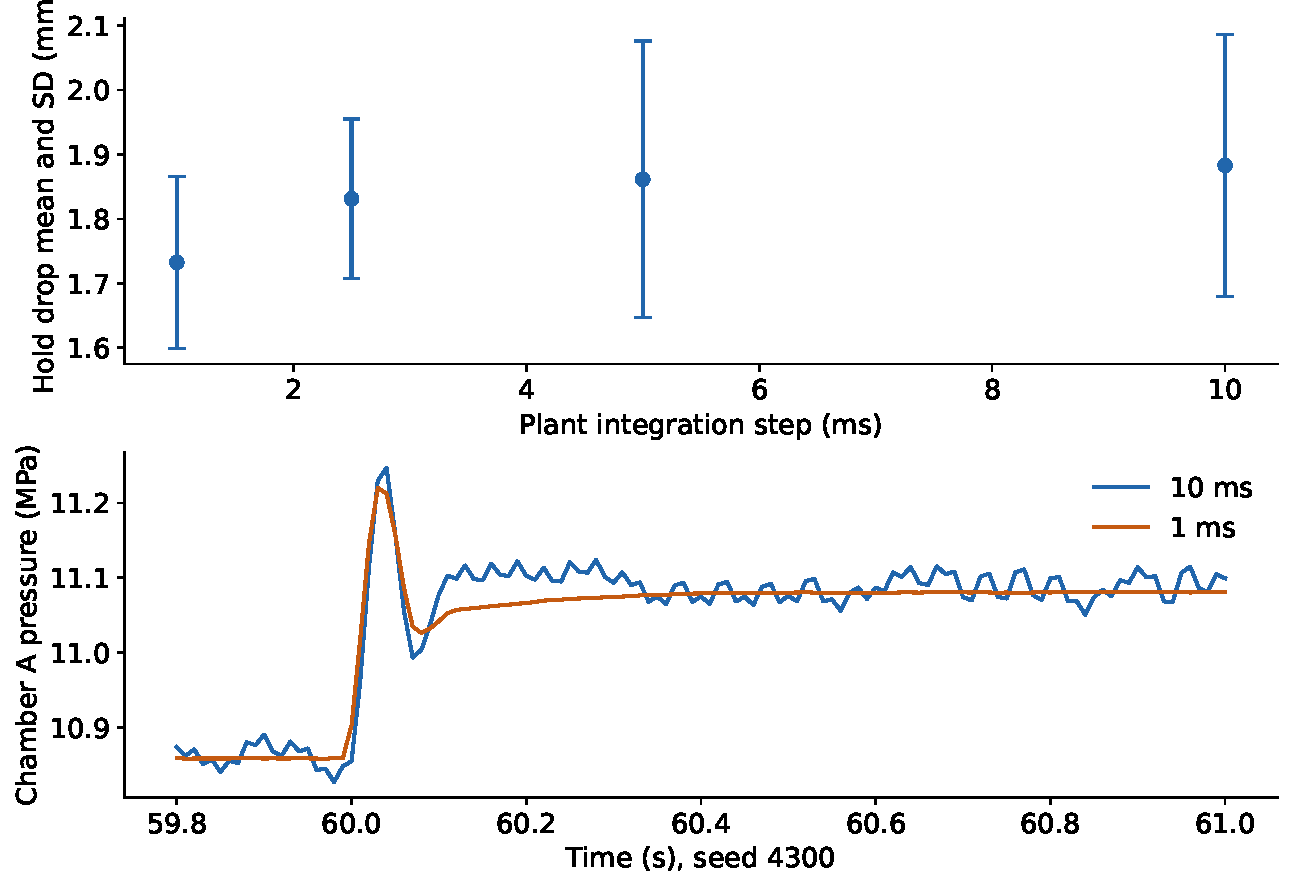
\includegraphics[width=1\linewidth]{revision_integration.pdf}
\caption{Plant-step
 sensitivity with unchanged controller/noise timing. The~upper panel shows mean and sample SD; the lower panel resolves the chamber-A pressure response near the load step for seed~4300.}\label{fig:integration}
\end{figure}

\vspace{-6pt}

\begin{table}[H]
\caption{Paired RK4 comparison on five common seeds per row, with~frozen gains and 10 ms sensing/control. The~matched PID arm adds an 8 s latch and discharge gating. RMSE is post-transition tracking error; oil is accumulator~discharge.}
\label{tab:rk4-comparators}
\small

\begin{adjustwidth}{-\extralength}{0cm}

\begin{tabularx}{\fulllength}{l cc  CCCC}
\toprule
\textbf{Chain} & \textbf{Step (ms)} & \textbf{Pass} & \textbf{Mean Drop (mm)} & \textbf{Mean RMSE (mm)} & \textbf{Mean Oil (mL)} & \textbf{Mean Changes}\\\midrule
Observer hybrid & 1.0 & 5/5 & 1.628 & 1.178 & 0.00 & 13.0 \\
PID--accumulator & 1.0 & 5/5 & 3.002 & 0.249 & 29.31 & 40.6 \\
PID + matched latch & 1.0 & 5/5 & 3.028 & 0.249 & 27.94 & 3.0 \\
Observer hybrid & 0.5 & 5/5 & 1.585 & 1.192 & 0.00 & 13.0 \\
PID--accumulator & 0.5 & 5/5 & 2.943 & 0.251 & 29.91 & 42.6 \\
PID + matched latch & 0.5 & 5/5 & 2.953 & 0.251 & 28.50 & 3.0 \\
\bottomrule
\end{tabularx}
\end{adjustwidth}
\end{table}

\subsection{Mechanical Mismatch and Retained Failure~Boundaries}
Table~\ref{tab:mechanical} supplies the previously missing V2 mass, damping and stiffness variation runs. All six one-at-a-time perturbations passed five paths with the controller and observer coefficients fixed at their nominal values. The worst hold drop remained below 2.30 mm; the largest post-transition error was 9.32 mm. None of these paths required accumulator discharge. These are five-seed one-at-a-time numerical screens; they do not establish robustness over a full $\pm30\%$ uncertainty~box.

\begin{table}[H]

\caption{New V2 one-at-a-time mechanical mismatch tests. The~observer and control coefficients remain~nominal.}\label{tab:mechanical}
\small
\begin{tabularx}{\textwidth}{l c C C c}
\toprule
\textbf{Changed Plant Input} & \textbf{Pass} & \textbf{Worst Drop (mm)} & \textbf{Worst Error (mm) }& \textbf{Mean Oil (mL)} \\
\midrule
Mass $\times$0.7 & 5/5 & 1.95 & 8.92 & 0.0 \\
Mass $\times$1.3 & 5/5 & 2.00 & 8.92 & 0.0 \\
Damping $\times$0.7 & 5/5 & 2.08 & 8.94 & 0.0 \\
Damping $\times$1.3 & 5/5 & 2.04 & 8.91 & 0.0 \\
Stiffness $\times$0.7 & 5/5 & 2.30 & 8.53 & 0.0 \\
Stiffness $\times$1.3 & 5/5 & 2.06 & 9.32 & 0.0 \\
\bottomrule
\end{tabularx}
\end{table}


The simultaneous perturbation screen in Table~\ref{tab:joint-mechanical} extends the one-at-a-time checks to all eight declared mass/damping/stiffness vertices. It yields 40/40 passing paths; the largest hold drop is 2.009 mm and the largest post-transition error is 9.177 mm. The~controller and observer remain nominal and no failing path is discarded. Section~\ref{sec4.8} separately samples interior mechanical, hydraulic, friction and sensor inputs together; neither finite screen certifies the complete region or its worst~case.


\begin{table}[H]
\caption{Joint mechanical corner screen with the hybrid, five paired seeds per vertex and 1 ms RK4 integration. All controller/observer coefficients remain nominal. Ratios refer to true plant mass, damping and stiffness. Worst values include every~path.}
\label{tab:joint-mechanical}
\small
\begin{tabularx}{\textwidth}{cccc CCC}
\toprule
\boldmath{$m/m_0$} & \boldmath{$c/c_0$} & \boldmath{$k/k_0$} & \textbf{Pass} & \textbf{Worst Drop (mm)} & \textbf{Worst Error (mm)} & \textbf{Mean Oil (mL)}\\
\midrule
1.3 & 1.3 & 1.3 & 5/5 & 1.595 & 9.155 & 0.00 \\
1.3 & 1.3 & 0.7 & 5/5 & 1.756 & 8.352 & 0.00 \\
1.3 & 0.7 & 1.3 & 5/5 & 1.583 & 9.023 & 0.00 \\
1.3 & 0.7 & 0.7 & 5/5 & 1.692 & 8.284 & 0.00 \\
0.7 & 1.3 & 1.3 & 5/5 & 1.746 & 9.153 & 0.00 \\
0.7 & 1.3 & 0.7 & 5/5 & 2.009 & 8.351 & 0.00 \\
0.7 & 0.7 & 1.3 & 5/5 & 1.750 & 9.177 & 0.00 \\
0.7 & 0.7 & 0.7 & 5/5 & 1.965 & 8.372 & 0.00 \\
\bottomrule
\end{tabularx}
\end{table}

The friction-mismatch screen in Table~\ref{tab:friction-mismatch} directly changes the true plant while retaining nominal observer/controller coefficients. Both predeclared arms pass all five combined load/leakage paths. The~mean hold drop is 2.46--2.47 mm and the largest post-transition error is 8.65 mm. The~small difference between the two factors does not imply friction-insensitive physical behavior; it is evidence only for these selected virtual inputs and~seeds.

\begin{table}[H]

\caption{Predeclared friction-mismatch screen under repeated load changes and fivefold virtual leakage. All observer/controller coefficients remain nominal; the three true-plant friction terms are scaled~together.}\label{tab:friction-mismatch}
\small
\begin{tabularx}{\textwidth}{l c CCCCC}
\toprule
\textbf{True-Plant Friction} & \textbf{Pass} & \textbf{Mean Drop (mm)} & \textbf{Worst Drop (mm)} & \textbf{Worst Error (mm)} & \textbf{Mean Oil (mL)} & \textbf{Mean Switches}\\\midrule
0.7$\times$ nominal & 5/5 & 2.46 & 2.88 & 8.63 & 43.14 & 56.4\\
1.3$\times$ nominal & 5/5 & 2.47 & 2.99 & 8.65 & 37.09 & 55.8\\
\bottomrule
\end{tabularx}
\end{table}

The original $+2$ mm position-bias group remains an accuracy failure, reaching a \mbox{10.61 mm} worst post-transition error. A small hold drop alone does not establish true position accuracy under bias. Passing the selected mechanical perturbations does not remove this sensing~boundary.

\subsection{Noise Activation and Finite-Accumulator~Consequences}
\label{sec4.7}

Table~\ref{tab:noise} separates pressure-only noise from jointly doubled sensors. V2 passed all five pressure-only paths through 0.50 MPa SD, while at 1.00 MPa, only 2/5 passed; the worst post-transition error reached 10.65 mm. No stroke-boundary hit or relief activation occurred in this sweep. At~high noise, the dwell timer limits mode-switch counts near their maximum achievable rate, and~accumulator oil use approaches 450 mL on average. The~result is an accuracy/activity failure rather than the historical stroke-boundary~instability.

\begin{table}[H]

\caption{V2 pressure-only noise sweep with no external prefilter. Position-noise SD remains 1.5 mm; the internal observer is~retained.}\label{tab:noise}
\small
\begin{tabularx}{\textwidth}{l @{\hspace{1.5em}}c@{\hspace{1.5em}}c@{\hspace{1.5em}}c@{\hspace{1.5em}}c@{\hspace{1.5em}}c}
\toprule
\textbf{Pressure SD (MPa)} & \textbf{Pass} & \textbf{Worst Error (mm)} & \textbf{Switches} & \textbf{Oil (mL)} & \textbf{Min.} \boldmath{$p_g$} \textbf{(MPa)} \\
\midrule
0.05 & 5/5 & 8.93 & 13.0 & 0.0 & 14.00 \\
0.10 & 5/5 & 9.03 & 13.6 & 98.8 & 13.33 \\
0.20 & 5/5 & 9.11 & 90.4 & 298.0 & 12.20 \\
0.50 & 5/5 & 9.64 & 218.6 & 447.1 & 11.50 \\
1.00 & 2/5 & 10.65 & 221.0 & 454.1 & 11.47 \\
\bottomrule
\end{tabularx}
\end{table}


The original jointly doubled-noise group used 61.98 mL mean oil, compared with 1.02 mL nominal, because~noisy filtered position, velocity and pressure balance repeatedly request support. The~new five-path joint-noise replay used 39.92 mL on average and reached a minimum gas pressure of 13.55 MPa. Its difference from 61.98 mL reflects a different seed set, not a changed controller. The~nominal new paths did not discharge at all. Activation time, mode occupancy and the full accumulator-pressure trajectory in the reproduction files show that the larger relative ratio starts from near-zero nominal consumption; it does not imply sixtyfold depletion of initial storage. Position holding remained within the screen on all five joint-noise paths, with~a worst error of 9.44~mm.

To reproduce the historical destructive input level, the~V2 hybrid was also run on seeds 2060--2079 with 0.10 MPa independent raw pressure noise per chamber, no external prefilter, and~its internal observer retained. All 20 paths passed: the mean hold drop was \mbox{1.86 mm} and worst error 8.72 mm; mean accumulator discharge was 105.4 mL. The~historical reduced-order raw-pressure case instead reached a 500 mm worst error at the stroke boundary. Identical absolute noise SD and seed labels do not make the perturbation processes identical: the plants, reference paths, draw sequences and observer interfaces differ. Thus, V2 does not reproduce that stroke failure at 0.10 MPa, but~the change cannot be attributed solely to the chamber architecture. The~broader V2 sweep identifies its own accuracy failure at \mbox{1 MPa}; it does not claim universal noise~robustness.


Figure~\ref{fig:noise} contrasts the distinct measurement-noise interventions.
\begin{figure}[H]
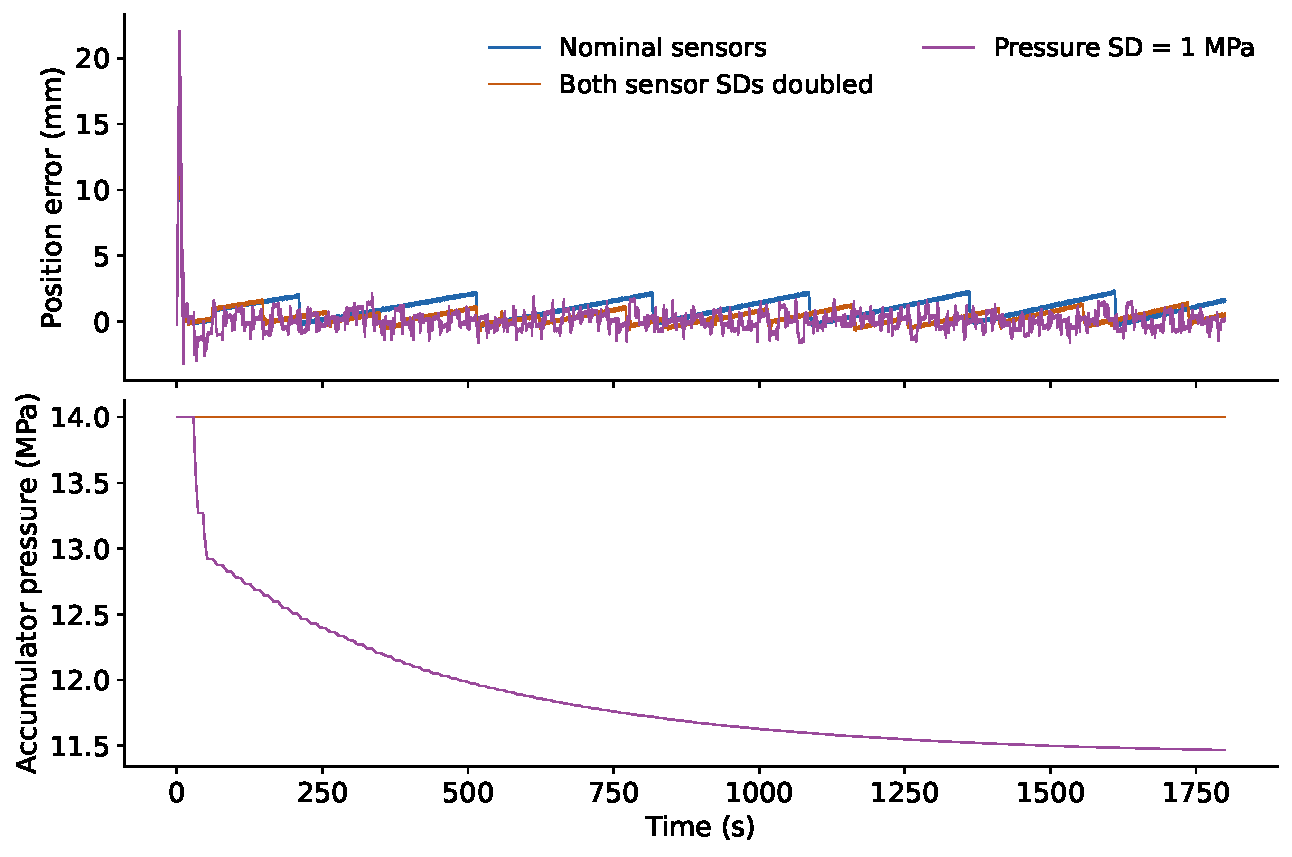
\includegraphics[width=0.83\linewidth]{revision_noise.pdf}
\caption{Position
 error and accumulator pressure over the complete predeclared seed-4300 trajectory. Jointly doubled noise and 1 MPa pressure-only noise are distinct interventions. Pressure-only SD is nominal in the first curve; the internal observer remains active in all~curves.}\label{fig:noise}
\end{figure}

All ten original jointly doubled-noise paths were additionally replayed with storage/activity logging; every originally recorded field reproduced exactly, including \mbox{61.98 mL} mean oil. Figure~\ref{fig:original-noise} shows the first original stress seed, 4160, against~a same-seed nominal replay. It resolves the support-command episodes and gas-pressure decline directly; the complete ten-path activity/storage summary is in \mbox{Supplementary S5}.

\begin{figure}[H]
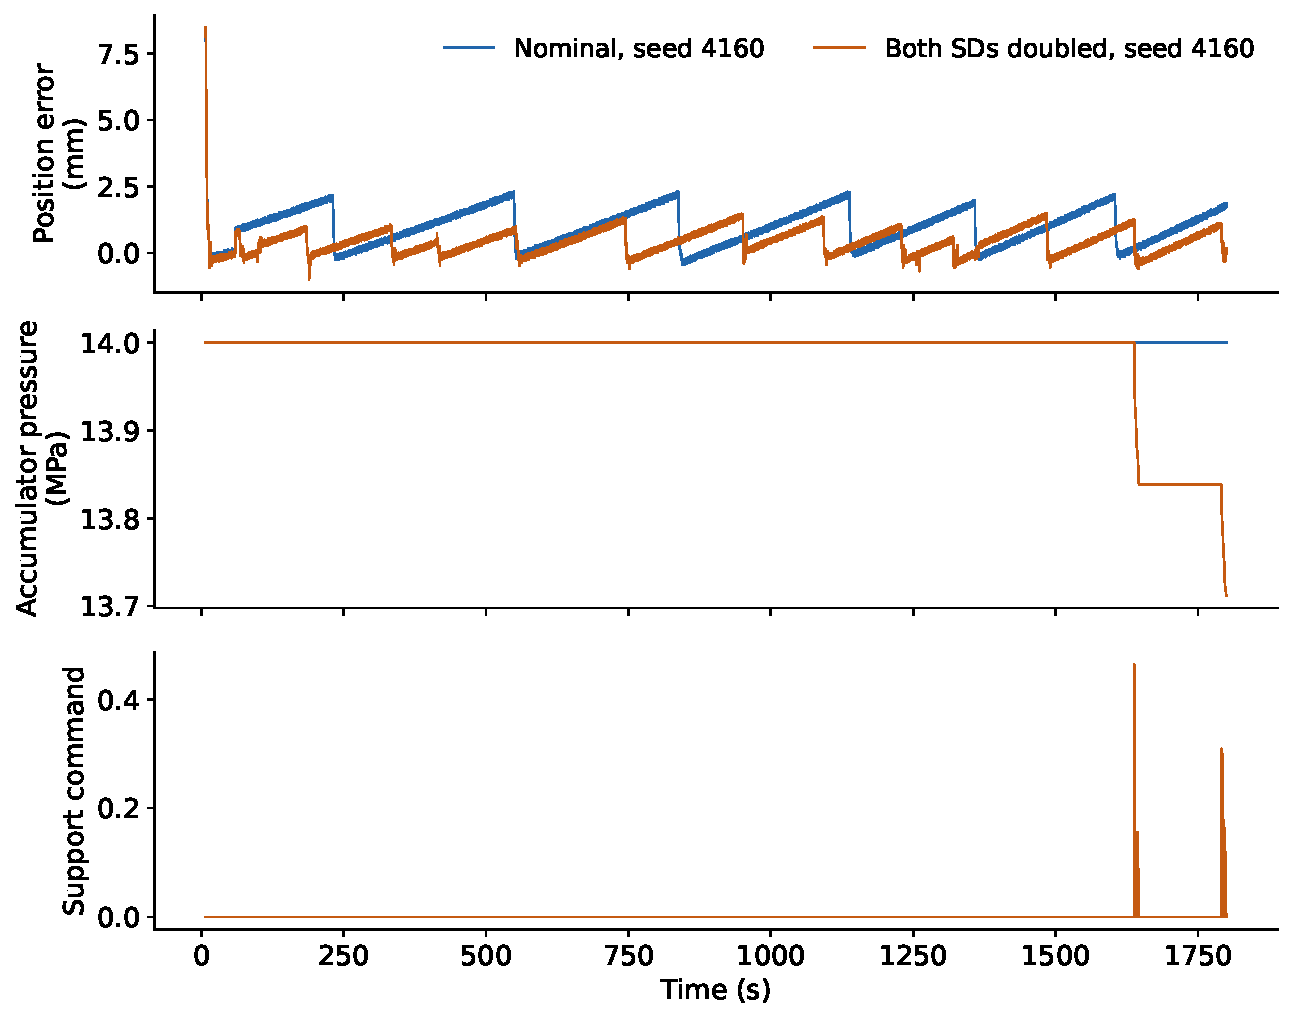
\includegraphics[width=0.83\linewidth]{revision_original_noise.pdf}
\caption{Original stress-group diagnosis: first frozen seed 4160, nominal versus jointly doubled sensors, after~the 8 s reference transition. The~doubled-noise path reproduces its original output fields. Curves display error, gas pressure and the support command rather than interpreting a relative oil-volume ratio as energy or storage~depletion.}\label{fig:original-noise}
\end{figure}


\subsection{Matched-Budget Independent Tests and Interacting~Uncertainty}
\label{sec4.8}




The refined combined-stress screen contains 30 paths. The~largest absolute paired hold-drop change between 1 and 0.5 ms is 0.250 mm. All individual outcomes are retained in Supplementary S10; proximity of the sampled accuracy screens does not establish fourth-order convergence at dry-friction or projection events. The~original 10 ms stress results remain identified as coarse-protocol~observations.

Table~\ref{tab:risk-convergence} summarizes the refined repeated-load audit.
\begin{table}[H]
\caption{Refined
 repeated-load stress audit with the submitted hybrid gains. Each row uses the same three seeds; controller timing remains 10~ms.}\label{tab:risk-convergence}
\small
\begin{tabularx}{\textwidth}{l C c C CC}
\toprule
\textbf{Stress Arm} & \textbf{Plant Step (ms)} & \textbf{Pass} & \textbf{Mean Drop (mm)} & \textbf{Worst Drop (mm)} & \textbf{Worst Error (mm)}\\\midrule
Nominal leakage & 1.0 & 3/3 & 2.118 & 2.714 & 8.421\\
Nominal leakage & 0.5 & 3/3 & 2.164 & 2.657 & 8.425\\
Fivefold leakage & 1.0 & 3/3 & 2.105 & 2.508 & 8.434\\
Fivefold leakage & 0.5 & 3/3 & 2.052 & 2.350 & 8.442\\
Fivefold, storage disabled & 1.0 & 3/3 & 2.229 & 2.510 & 8.434\\
Fivefold, storage disabled & 0.5 & 3/3 & 2.167 & 2.343 & 8.442\\
Fivefold, friction $0.7\times$ & 1.0 & 3/3 & 1.990 & 2.166 & 8.424\\
Fivefold, friction $0.7\times$ & 0.5 & 3/3 & 1.965 & 2.124 & 8.424\\
Fivefold, friction $1.3\times$ & 1.0 & 3/3 & 2.075 & 2.336 & 8.435\\
Fivefold, friction $1.3\times$ & 0.5 & 3/3 & 2.001 & 2.290 & 8.435\\
\bottomrule\end{tabularx}\end{table}


The development rule selects $(g_t,g_a)=(1.0,0.5)$ for the hybrid and $(1.3,0.5)$ for matched PID. Table~\ref{tab:risk-validation} reports the independent data, while Figure~\ref{fig:risk-frontier} shows every development candidate. Selection uses the declared scalar preference; the nondominated points expose alternative tracking, holding, discharge and switching~compromises.

\begin{table}[H]
\caption{Independent full-duration evaluation after equal-budget development. The~selected policies use common sensing, authority, dwell, load and leakage. Means are reported; there are ten independent seeds per~row.}\label{tab:risk-validation}
\small

\begin{tabularx}{\textwidth}{l c@{\hspace{1.95em}}c@{\hspace{1.95em}}c@{\hspace{1.95em}}c@{\hspace{1.95em}}c@{\hspace{1.95em}}c}\toprule
\textbf{Policy} & \textbf{Step (ms)} & \textbf{Pass} & \textbf{Drop (mm)} & \textbf{RMSE (mm)} & \textbf{Oil (mL)} & \textbf{Changes}\\\midrule
Hybrid & 1.0 & 10/10 & 2.181 & 1.262 & 23.97 & 54.5\\
Hybrid & 0.5 & 10/10 & 2.109 & 1.273 & 23.79 & 54.2\\
Matched PID & 1.0 & 10/10 & 3.646 & 0.310 & 34.76 & 7.0\\
Matched PID & 0.5 & 10/10 & 3.556 & 0.314 & 35.29 & 7.0\\
\bottomrule\end{tabularx}\end{table}

At 0.5 ms, the selected hybrid passes 10/10 and matched PID passes 10/10. Their mean hold drops are 2.109/3.556 mm, tracking RMSE 1.273/0.314 mm, discharge \mbox{23.79/35.29 mL}, and~changes 54.2/7.0. Paired differences and uncertainty intervals are given in \mbox{Supplementary S10}. These data quantify the chosen policies rather than establishing algorithm-wide~superiority.

Disabling storage in the selected hybrid at 1 ms gives 10/10 passing paths, a mean drop of 2.206 mm and worst error of 8.469 mm. Together with the frozen-gain ablation, this does not establish that storage is necessary. The~evaluated contribution is therefore the observation/supervision protocol and its explicit trade-offs; no indispensable accumulator or energy-saving claim is~made.

The 24-path interacting-uncertainty screen has 22/24 passing paths. Its worst sampled post-transition error is 10.155 mm and worst defined hold drop is 3.659 mm. Counts of failed criteria can overlap: zero paths fail to enter hold, two exceed the 10 mm error screen, zero exceed the drop screen, zero activate relief and zero reach a stroke boundary. All sampled inputs and outcomes are retained, including failures. This finite design supplies interaction evidence and a failure boundary, not a certified uncertainty region or physical success~probability.


\begin{figure}[H]
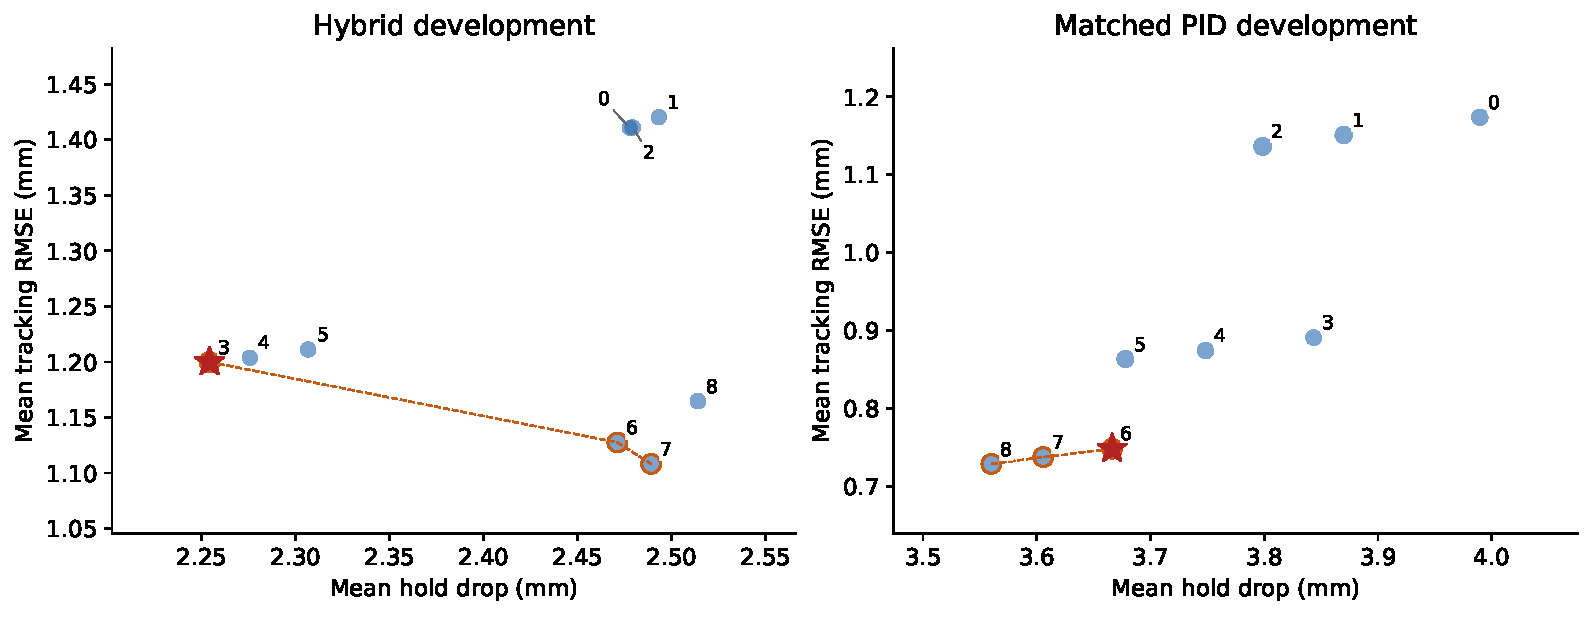
\includegraphics[width=\linewidth]{risk_closure_frontier.pdf}\caption{Equal-budget
 development: all nine candidates per policy. Connected outlines identify the projection of the four-objective nondominated subset; they are not an interpolated attainable frontier. Blue circles denote all candidates; orange outlined circles and dashed connections identify the nondominated subset in each panel. Red stars denote the frozen scalar-rule selections.}\label{fig:risk-frontier}\end{figure}

\vspace{-9pt}

Figure~\ref{fig:risk-validation} displays the paired validation paths and interacting-uncertainty screen.
\begin{figure}[H]
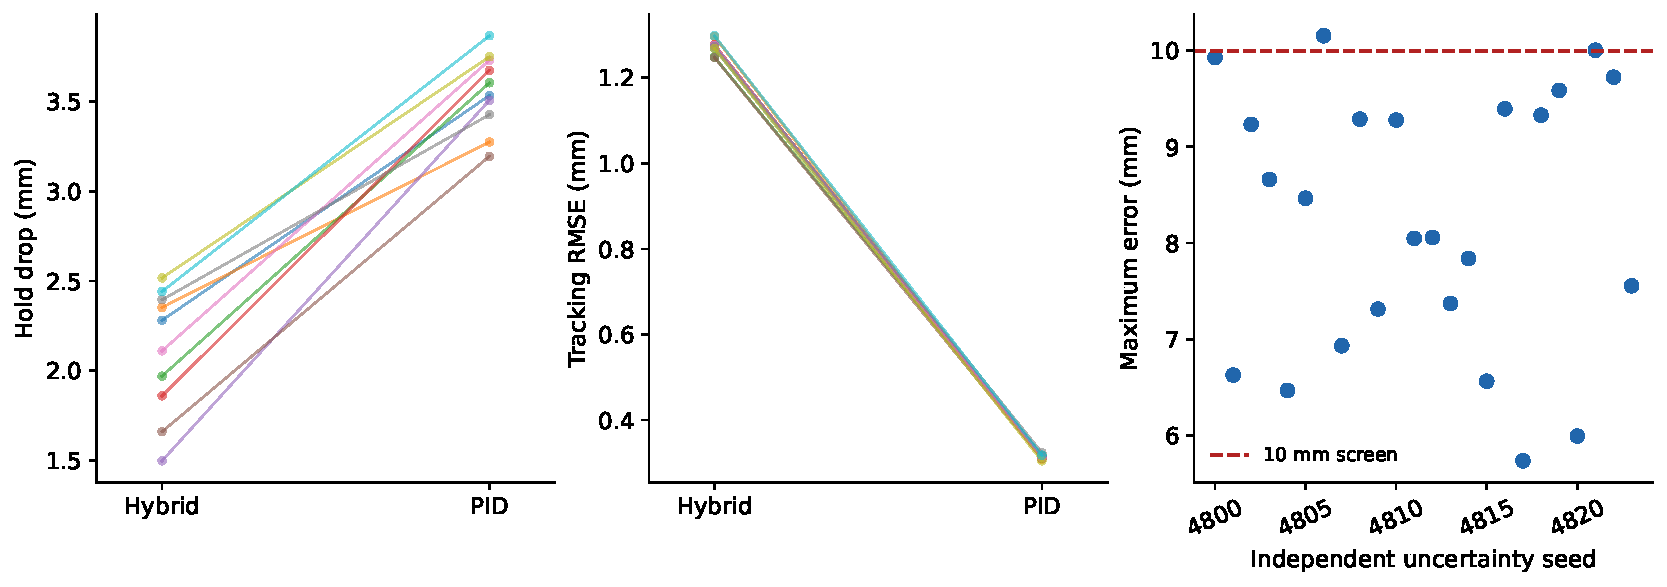
\includegraphics[width=\linewidth]{risk_closure_validation.pdf}\caption{Independent
 selected-policy comparisons and the separate 24-path interacting-uncertainty screen. Each colored line in the first two panels connects the hybrid and PID outcomes for one common seed; colors distinguish seeds, not policies. Blue points in the third panel denote the separate uncertainty paths; the red dashed line marks the 10 mm screen. The uncertainty panel retains every new~sample.}\label{fig:risk-validation}\end{figure}



\subsection{Active Nonlinear Comparison and Accuracy-Margin~Validation}
\label{sec4.9}

Table~\ref{tab:extension-nominal} summarizes the execution-verified nominal comparison. The execution-verified SMC development selects $(g_t,g_a)=(1.3,0.5)$. It passes 10/10 and 10/10 common nominal paths at 1 and 0.5 ms, respectively. The~earlier unlatched SMC data are not used in this matched comparison. The~corrected SMC passes 24/24 on known vectors and 24/24 on the previous 4900-series joint design. The~scalar hybrid/PID/margin outcomes on that previous design remain 23/24, 24/24 and 24/24. These are follow-up checks on known protocols; Table~\ref{tab:extension-fresh} instead reports the newly frozen 5100-series~design.

\begin{table}[H]

\caption{Execution-verified
 repeated-load/fivefold-leakage comparison at 0.5 ms RK4. All four instances use common seeds 4700--4709. These are paired follow-up results; corrected SMC receives an explicit 8 s latch and discharge gate. Means are~shown.}\label{tab:extension-nominal}
\small
\begin{tabularx}{\textwidth}{l CCCCC}\toprule
\textbf{Policy} & \textbf{Pass} & \textbf{Drop (mm)} & \textbf{RMSE (mm)} & \textbf{Oil (mL)} & \textbf{Changes}\\\midrule
Scalar hybrid & 10/10 & 2.109 & 1.273 & 23.79 & 54.2\\
Active PID & 10/10 & 3.556 & 0.314 & 35.29 & 7.0\\
Active SMC & 10/10 & 1.992 & 0.251 & 13.62 & 5.6\\
Margin hybrid & 10/10 & 2.026 & 1.204 & 153.15 & 54.0\\
\bottomrule\end{tabularx}\end{table}

On the new joint design, scalar hybrid/PID/corrected active SMC/margin hybrid pass 24, 24, 24 and 24 of 24 paths, respectively. The~margin hybrid's worst sampled error is \mbox{8.544 mm} and worst hold drop is 3.109 mm. Its earlier 4900-series result of 24/24 and \mbox{8.569 mm} remains a result for that previous design, not a substitute for this new test. Figure~\ref{fig:extension-fresh} displays every new path. Supplementary S11 supplies all development candidates, exact failed seeds, both nominal steps and paired descriptive~intervals.

\begin{table}[H]
\caption{New simultaneous parameter/friction/sensing design, seeds 5100--5123, at~1 ms RK4. All four frozen instances face the same 24 vectors and noise sequences. Worst error and other-metric means include every path with defined values; failed paths are~retained.}\label{tab:extension-fresh}
\small
\begin{tabularx}{\textwidth}{l c C cc c c}\toprule
\textbf{Policy} & \textbf{Pass} & \textbf{Worst Error (mm)} & \textbf{Drop (mm)} & \textbf{RMSE (mm)} & \textbf{Oil (mL)} & \textbf{Changes}\\\midrule
Scalar hybrid & 24/24 & 9.972 & 2.419 & 1.381 & 175.10 & 73.5\\
Active PID & 24/24 & 7.068 & 3.869 & 1.076 & 34.11 & 7.0\\
Active SMC & 24/24 & 7.377 & 2.042 & 1.056 & 13.79 & 5.8\\
Margin hybrid & 24/24 & 8.544 & 2.134 & 1.276 & 245.34 & 88.2\\
\bottomrule\end{tabularx}\end{table}



All four instances pass every new joint path. This new design therefore does not demonstrate an additional pass-rate benefit from the margin requirement; the previous-design scalar failure remains separately~reported.

The reserve's nominal stored-fluid cost remains substantial: scalar/margin mean discharge is 23.79/153.15 mL. Corrected active SMC has nominal mean drop 1.992 mm, RMSE 0.251 mm, discharge 13.62 mL and 5.6 mode changes. Thus, all four objectives, including costs introduced by the accuracy-oriented preference, must be compared together. Accumulator discharge does not measure total input~energy.

Corrected active SMC has lower nominal means on all four objectives than both hybrid variants and the active PID. Thus, this matched nominal test supplies no mean-objective performance advantage for either hybrid. Lower means alone do not imply statistically established dominance of every objective or a universal controller ranking; paired intervals against corrected SMC are supplied in Supplementary S11. The~scalar hybrid's smaller discharge relative to PID remains a comparator-specific result and cannot be extended to~SMC.

The same four-mean ordering favors corrected SMC over both hybrids on the new joint design. This is a negative result for a hybrid-performance claim, not evidence that one controller wins on every metric: the active PID has a smaller sampled worst error than~SMC.

Successful finite screens do not certify the twelve-dimensional interval. Gaussian noise has no finite deterministic bound, the~friction function remains fixed, and~the margin is a declared development requirement rather than an observer-error theorem. The~current comparison evaluates policy instances under explicit choices; it does not establish universal hybrid~superiority.





\subsection{Supply Availability and the Storage~Contribution}\label{sec:supply-results}
\label{sec4.10}

The additional supply experiment evaluates previously frozen gains, with~a newly declared boundary-resource measurement. It does not replace the four-objective negative comparison in Section~\ref{sec4.9}. Table~\ref{tab:supply-normal} and Figure~\ref{fig:supply-normal} report all four normal-supply seeds; the availability hybrid is numerically identical to the scalar hybrid on these~paths.

\begin{table}[H]
\caption{New normal-supply repeated-load paths, seeds 5500--5503, 1 ms RK4. Means use the common 8.01--1800 s window. B is the declared boundary-resource index, not total input energy. All four paths enter holding under each~policy.}\label{tab:supply-normal}
\small
\begin{tabularx}{\textwidth}{l CCCC c}\toprule
\textbf{Policy} & \textbf{Pass} & \textbf{RMSE (mm)} & \boldmath{$V_s$} \textbf{(mL)} & \textbf{Oil (mL)} & \boldmath{$B$} \textbf{(kJ)}\\\midrule
Scalar hybrid & 4/4 & 1.271 & 1085.0 & 21.55 & 23.08\\
Active PID & 4/4 & 0.314 & 1592.7 & 34.58 & 33.93\\
Active SMC & 4/4 & 0.252 & 13405.7 & 13.49 & 281.71\\
Availability hybrid & 4/4 & 1.271 & 1085.0 & 21.55 & 23.08\\
\bottomrule\end{tabularx}\end{table}

Scalar hybrid/active SMC mean main-supply volume is 1085.0/13,405.7 mL and mean B is 23.08/281.71 kJ. Their RMSE is 1.271/0.252 mm. The~relative main-supply-volume difference, 91.91\%, is a ratio of these group means. It quantifies a resource--tracking trade-off at frozen gains; it is not an energy-saving rate or evidence that SMC cannot reach a different trade-off after resource-oriented retuning. Supplementary S12 gives the paired differences. The~earlier four-objective ordering favoring SMC remains~valid.

\begin{figure}[H]


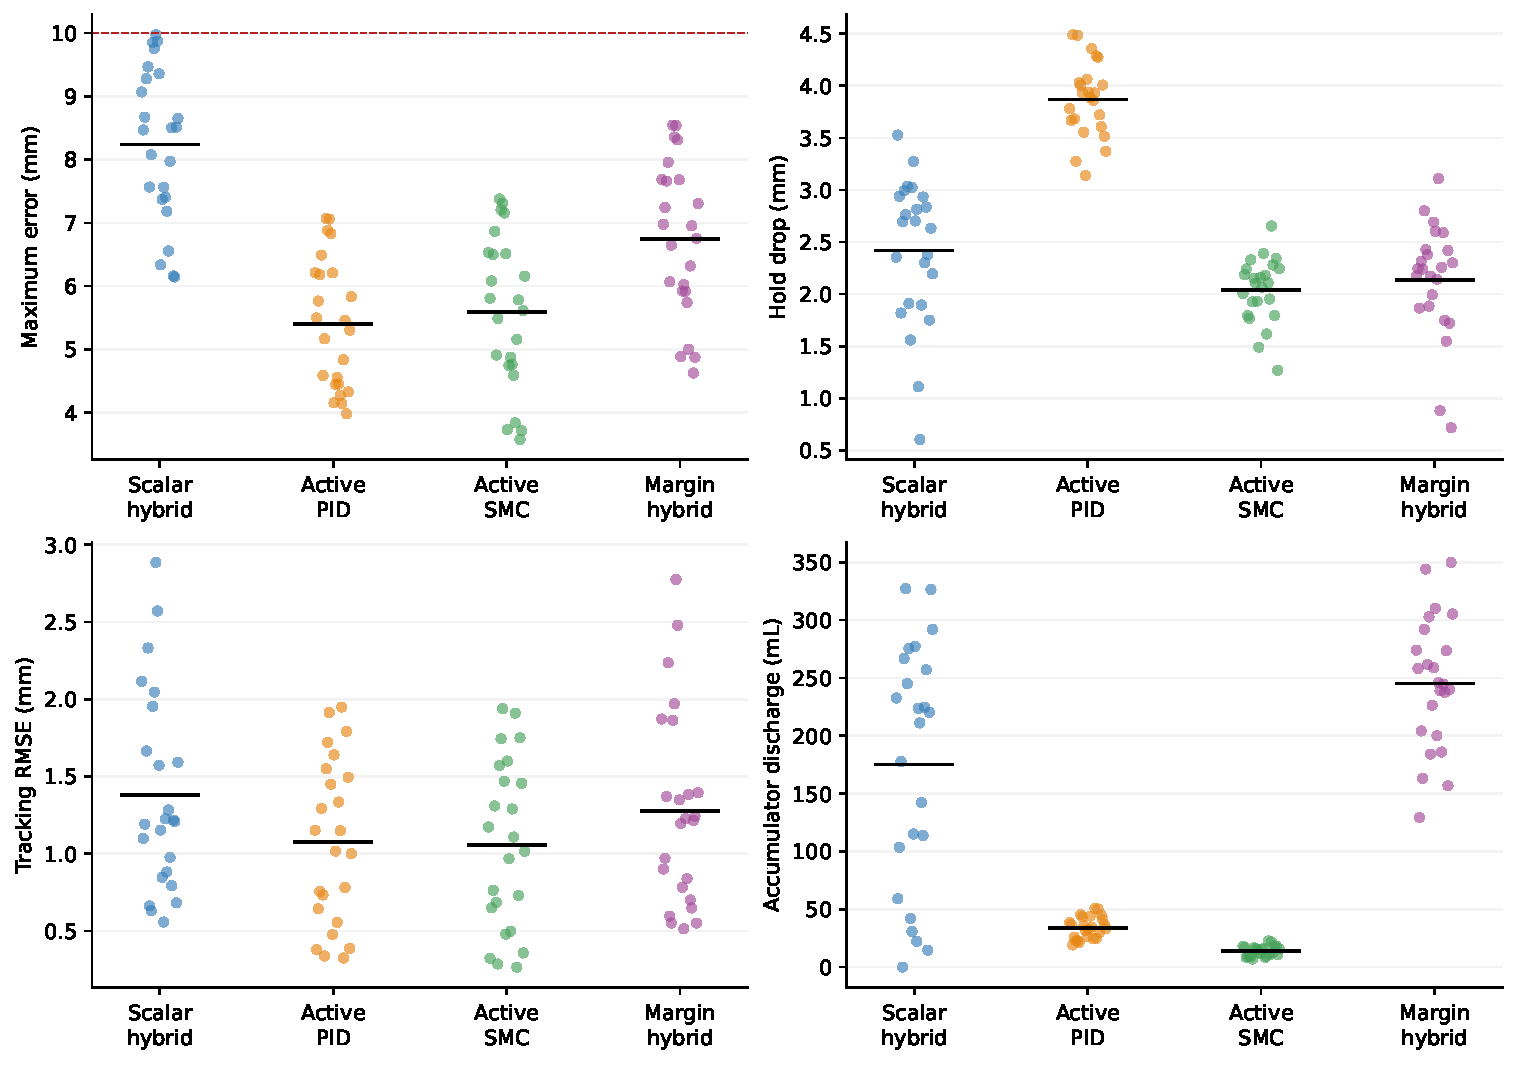
\includegraphics[width=12 cm]{risk_extension_fresh.pdf}

\caption{New
 simultaneous uncertainty, seeds 5100--5123: all 24 paired vectors under each frozen policy with verified baseline latch/gating. Points show individual paths; black bars show means. The red dotted line marks the 10 mm maximum-error screen. The~10 mm threshold applies to maximum error, not RMSE. Discharge is stored-fluid use rather than system~energy.}\label{fig:extension-fresh}\end{figure}

\vspace{-9pt}

\begin{figure}[H]

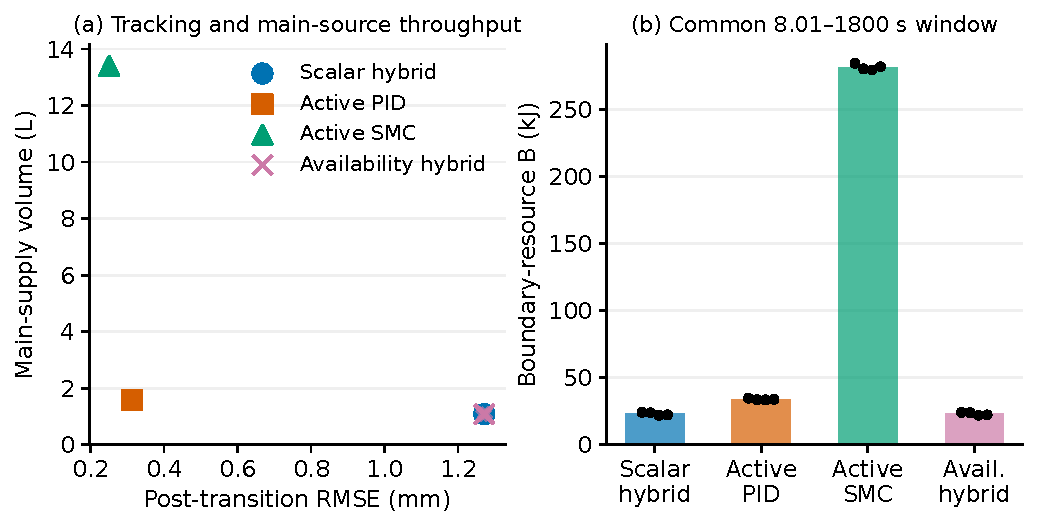
\includegraphics[width=11.5 cm]{risk_extension_supply_normal.pdf}
\caption{Normal-supply
 resource and tracking comparison. (a) Smaller colored markers denote the four seeded paths and larger markers denote policy means; some markers overlap. (b) Colored bars denote mean boundary resource and black dots denote individual paths.
 The~two hybrid instances coincide because the availability extension is inactive. $B$
 includes main-source and storage-outlet work only; no pump-input or efficiency claim~follows.}\label{fig:supply-normal}\end{figure}

For the eight new joint vectors with supply disconnected on [300,1500) s, complete-path pass counts are scalar hybrid: 8/8 with storage and 1/8 without; active PID: 8/8 with storage and 1/8 without; active SMC: 8/8 with storage and 0/8 without; availability hybrid: 8/8 with storage and 1/8 without. Figure~\ref{fig:supply-interruption} includes every on/off outcome; passing requires hold entry, both 10 mm screens, and~no relief or stroke event. The~current availability signal is ideal and all policies retain the same return~path.

Within this storage-enabled joint family, the scalar hybrid/active SMC mean main-source volume is 539.9/4903.6 mL and B is 15.02/110.12 kJ. These separately paired resource comparisons are reported in Supplementary S12; their schedules differ from the normal repeated-load~family.

The availability hybrid's worst sampled post-transition error is 9.215 mm and worst confirmed-hold drop is 2.051 mm. Mean within-interruption maximum error is 1.173 mm, compared with 3.571 mm for the scalar hybrid; the complete-path screen still includes the earlier transition. The mean storage use is 409.74/286.68 mL, respectively. Paired changes are given in Supplementary S12. This small fixed design evaluates the stated availability rule and does not establish a superior controller~family.

At fixed plant and noise inputs, enabling storage changes a failed complete path into a passing path in scalar hybrid: 7/8, active PID: 7/8, active SMC: 8/8, availability hybrid: 7/8. The~reverse changes, unchanged pass/fail cases and exact seeds are also retained in Supplementary S12. Storage necessity is therefore judged for each declared policy and interruption, while the original continuously supplied disabled-storage successes remain valid. A~common pass ratio cannot establish physical reliability or universal~necessity.

\begin{figure}[H]


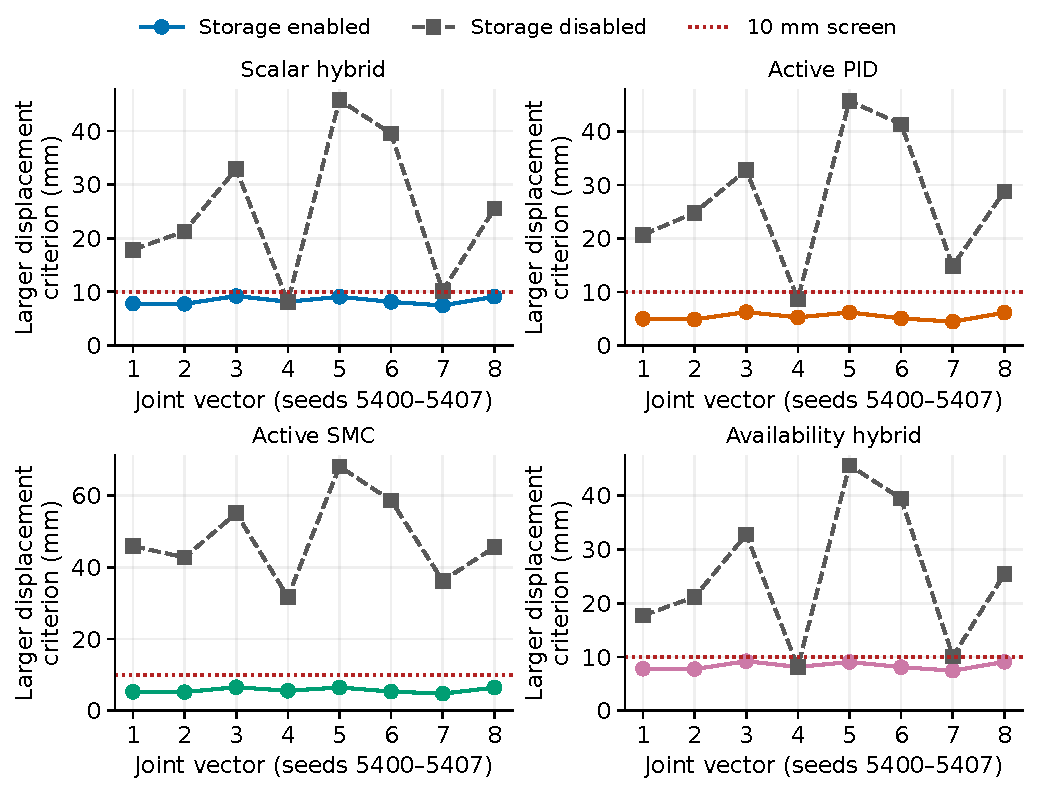
\includegraphics[width=11.5 cm]{risk_extension_supply_interruption.pdf}

\caption{All
 eight paired joint vectors during the 1800 s supply-availability study. Solid circles in blue, orange, green and purple identify storage-enabled scalar hybrid, PID, SMC and availability hybrid, respectively; gray dashed squares identify storage-disabled paths. Red dotted lines mark the 10 mm screen. Each value is the larger of maximum post-transition absolute error and confirmed-hold drop; both have the same \mbox{10 mm} limit. Thus, an error below 10 mm alone cannot hide a drop failure. Maximum error includes the pre-interruption transition. Other pass conditions and all failed seeds are reported in Supplementary S12.}\label{fig:supply-interruption}\end{figure}

The prespecified seed-5400 refinement gives a largest absolute drop change of \mbox{0.212 mm} and maximum-error change of 0.195 mm across the eight policy/storage pairs. Pass status changes in zero of eight pairs. This is a representative numerical sensitivity check, not convergence certification over all joint~vectors.

The archived both-port-isolation exploration provides an adverse mechanism check: all eight 600 s interruption paths fail the 10 mm screen, including storage-enabled paths. Added storage alone cannot supply the required return balance, and~gas--A pressure equalization can stop useful discharge while oil remains. That failed boundary is distinct from Equation~\eqref{eq:supply-flow}. The~prospectively frozen supply-only results do not repair or replace those~failures.

\subsection{Resource-Oriented Retuning of the Active~Comparison
}\label{sec:resource-retuning}

The additional search replaces the earlier four-objective selection criterion only for this separate experiment. It leaves the earlier trajectories and negative SMC comparison unchanged. Both policies receive 27 complete development paths and four independent validation paths. Table~\ref{tab:resource-retuning} reports means and sample standard deviations for all four validation paths per policy; Supplementary S13 retains the complete candidate ranking and per-seed~records.

\begin{table}[H]
\caption{Independent normal-supply validation after equal-budget resource-oriented selection, seeds 5620--5623. Continuous metrics are mean $\pm$ sample SD across four paths per policy ($n-1=3$ in the variance denominator). $B$, RMSE and $V_s$ use endpoints 8.01--1800 s; $V_{acc}$ is total path discharge and drop uses confirmed hold. $B$ is boundary work accounting, not total input~energy.}\label{tab:resource-retuning}
\small
\begin{tabularx}{\linewidth}{@{}>{\raggedright\arraybackslash}p{.44\linewidth}*{2}{>{\centering\arraybackslash}X}@{}}\toprule
\textbf{Metric} & \textbf{Scalar Hybrid} & \textbf{Active SMC}\\\midrule
Selected $(g_t,g_a)$ & (1.3,0.3) & (0.7,0.5)\\
Complete paths passing & 4/4 & 4/4\\
Boundary resource $B$ (kJ) & 22.47 $\pm$ 0.26 & 209.32 $\pm$ 2.39 \\
Post-transition RMSE (mm) & 1.2083 $\pm$ 0.0115 & 0.3086 $\pm$ 0.0006 \\
Stored-oil discharge $V_{acc}$ (mL) & 104.00 $\pm$ 15.43 & 35.96 $\pm$ 2.15 \\
Main-source volume $V_s$ (mL) & 1002.1 $\pm$ 17.8 & 9943.6 $\pm$ 114.1 \\
Confirmed-hold drop (mm) & 2.481 $\pm$ 0.211 & 2.754 $\pm$ 0.158 \\
Mode changes & 55.0 $\pm$ 0.0 & 7.0 $\pm$ 0.0 \\
\bottomrule\end{tabularx}\end{table}

The selected hybrid/SMC gain pairs are (1.3,0.3)/(0.7,0.5). They pass 4/4 and 4/4 validation paths. Mean $B$ is 22.47/209.32 kJ, while RMSE is 1.208/0.309 mm. Worst sampled maximum error is 7.022/9.913 mm. Mean stored-oil discharge is 104.00/35.96 mL and mean mode changes are 55.0/7.0; lower boundary resource does not imply lower storage use or activity. Both selected instances are development-feasible; validation is reported without reselection. Their differing RMSE prevents an equal-accuracy efficiency claim. The~common gain search tests the resource comparison within its declared range; it cannot exclude improved SMC settings outside that range or under changes to the nonlinear term. The~earlier and new validation seed sets differ, so cross-experiment mean changes are not paired causal estimates of retuning. No percentage is interpreted as total-energy~saving.


Table~\ref{tab:comparison-map} consolidates the controller versions and experiment protocols.
\begin{table}[H]
\caption{Controller
 versions and protocols for the principal comparisons in Sections~\ref{sec4.1} and \ref{sec4.8}--\ref{sec:resource-retuning}. All controller/observer periods are 10 ms. Gain multipliers $(g_t,g_a)$ and objective $J$ are defined in Section~\ref{sec3.6}. The~SMC force parameters remain 1200 N, 18 s$^{-1}$ and 0.006 m s$^{-1}$ (Section \ref{sec3.3}). Seed ranges denote different experiment roles, not pooled~replicates.}\label{tab:comparison-map}
\footnotesize
\begin{tabularx}{\textwidth}{LLLL}
\toprule
\textbf{Section and Versions} & \textbf{Objective and Adopted Gains} & \textbf{Development Inputs} & \textbf{Principal Evaluation and Plant Step}\\\midrule
Section

 \ref{sec4.1}: original PID--lock, SMC--lock, PID--accumulator \mbox{and hybrid} & Frozen tracking gains 650, 90; PID integral 20. PID storage gain 80; hybrid storage gains 1.5 and 60. Hybrid supervisor: 8 s, 4 mm, 0.30 MPa. & Hybrid only: 27 supervisor tuples; 4100--4104, 300 s. Rank by pass count, oil, changes, drop. Other original gains fixed. & 4120--4139, 1800 s, single load step; sequential explicit plant update, \mbox{10 ms}. Independent original audit: 4200--4219.\\
\midrule
Section \ref{sec4.8}: scalar hybrid and matched PID & Failures, then four-objective $J$. Hybrid $(1,0.5)$; PID $(1.3,0.5)$. Common authority and 8 s latch/gate. & Nine pairs each: $g_t=0.7,1,1.3$; $g_a=0.5,1,1.5$. Seeds 4600--4602, 300 s, \mbox{RK4 1 ms}. & Independent 4700--4709, 1800 s repeated loads, $5\times$ leakage; \mbox{RK4 1/0.5 ms}. Submitted-gain joint screen: 4800--4823, \mbox{RK4 1 ms}.\\


\bottomrule
\end{tabularx}

\end{table}

\begin{table}[H]\ContinuedFloat

\caption{\textit{Cont.}}



\footnotesize
\begin{tabularx}{\textwidth}{LLLL}
\toprule
\textbf{Section and Versions} & \textbf{Objective and Adopted Gains} & \textbf{Development Inputs} & \textbf{Principal Evaluation and Plant Step}\\\midrule




Section \ref{sec4.9}: scalar hybrid, active PID, corrected active SMC and margin hybrid & Same $J$; corrected SMC $(1.3,0.5)$. Scalar/PID gains as 4.8. Margin hybrid $(1.3,0.5)$: require development \mbox{error $\le8$ mm} before $J$. & Same nine-pair grid and 4600--4602. Corrected SMC development actually applies the 8 s latch and discharge gate; 300 s, RK4 1 ms. & Common 4700--4709 at RK4 1/0.5 ms; known 4800/4900-series follow-ups. New joint verification: 5100--5123, 1800 s, RK4 1 ms.\\
\midrule
Section \ref{sec4.10}: scalar and availability hybrids; active PID and SMC & No resource-based reselection. Hybrid variants $(1,0.5)$; PID/SMC $(1.3,0.5)$. Availability thresholds are fixed as in Section~\ref{sec:supply-method}. & Inherit 4.8/4.9 gains. Exploratory 5200--5202 records remain separate from prospective tests. & Normal supply: 5500--5503, repeated loads. Interruption [300,1500) s: joint 5400--5407, storage on/off. 1800 s, RK4 1 ms; seed 5400 also 0.5 ms.\\
\midrule
Section \ref{sec:resource-retuning}: resource-selected scalar hybrid and active SMC & Failures, then mean boundary resource $B$, then ID. Hybrid $(1.3,0.3)$; SMC $(0.7,0.5)$. & Nine pairs each: $g_t=0.7,1,1.3$; $g_a=0.3,0.5,0.7$. Seeds 5600--5602, complete 1800 s paths, RK4 1 ms. & Independent 5620--5623, normal supply, repeated loads, $5\times$ leakage, \mbox{1800 s}, RK4 1 ms. No joint-uncertainty validation in this family.\\\bottomrule
\end{tabularx}
\end{table}
\unskip


\section{Discussion}
\unskip
\subsection{Supported Contribution and Comparator~Choice}
The contribution is a reproducible holding-supervision experiment under explicit sensing, storage and numerical assumptions. It does not establish a new observer or hydraulic robust-control theorem. Four complete chains, rather than three, are compared in the original V2 experiment: PID--lock, sliding-mode--lock, PID--accumulator and observer hybrid. The~first two isolate the consequences of holding with the main valve locked; PID--accumulator supplies an active compensation baseline. The~latter has lower tracking RMSE and passes the same screen, making it an informative comparator rather than a deliberately weak failing~arm.

Adaptive robust control, backstepping, disturbance-observer control and dead-zone compensation provide important alternatives~\cite{yao2000,guan2008,choux2010,deng2017,chen2016}. Each would require a specified observer, saturation treatment, hold-entry policy and a fair tuning budget on this plant. Complete implementations of those adaptive or compensation designs remain outside the current comparison; the additional active boundary-layer sliding-mode chain has the narrower scope stated in Section~\ref{sec3.6}. No claim of superiority over mainstream electrohydraulic control follows. The~matched-timer test also rules out a broad switching-activity superiority claim. A smaller hold drop and lower accumulator discharge relative to the evaluated active PID instances come with a tracking-accuracy cost. The~active nonlinear comparison must be assessed separately across all reported~metrics.

The original-gain paired RK4 experiment retains that trade-off at both 1.0 and 0.5 ms under common measurement timing and seeds. At~0.5 ms, the~hybrid has 1.585 mm mean drop and 1.192 mm RMSE, compared with 2.953 mm and 0.251 mm for the matched-latch PID. Mean accumulator discharge is zero versus 28.50 mL, while the matched PID still switches less often (3.0 versus 13.0 changes). These original-gain results remain conditional on their implemented tuning. The~additional equal-budget comparison in Section~\ref{sec4.8} examines that dependence with common authority, a~declared objective and independent test seeds; it does not optimize a complete continuous frontier. Discharged oil is not total hydraulic~energy.

The execution-verified SMC follow-up in Section~\ref{sec4.9} keeps nonlinear compensation active during holding and explicitly applies the baseline latch/discharge gate. Its corrected development selection is separated from the new 5100-series joint verification. Earlier unlatched outputs remain diagnostic history and do not support a matched-comparison claim. Corrected SMC has lower nominal means on all four objectives than both hybrids and PID. The~hybrid--PID trade-off therefore cannot establish a hybrid advantage against this stronger active comparator. The~contribution is the documented coordination/attribution experiment and its limitations, not a demonstrated performance improvement over every evaluated policy. The~scalar-selected and margin-selected hybrids remain distinct preferences with unchanged gains. Common nominal seeds support paired follow-up comparisons, while the newly frozen joint vectors provide a separate evaluation. No favorable endpoint retroactively redefines a previous~holdout.

Section~\ref{sec:supply-results} adds a resource measurement missing from that four-objective comparison. At~the frozen gains, lower main-source throughput accompanies the scalar hybrid's larger tracking error. Section~\ref{sec:resource-retuning} separately tests this comparison after equal-budget gain selection for the boundary-resource index. Its finite grid and differing tracking errors preclude a globally optimal or equal-accuracy efficiency claim. The~availability extension is an incremental coordination rule whose benefit is restricted to the declared supply boundary. Its lower within-interruption error consumes more stored oil, and~the earlier transition still determines its complete-path maximum error. Because~both command allocation and support thresholds change together, these tests do not isolate the value of the availability signal~alone.

The storage contrast has a separate scope. Under~continuously supplied conditions, disabling storage can leave every tested path passing. Under~the new supply-disconnection design, enabled storage changes seven of eight failed scalar/availability-hybrid paths into passing paths at matched plant and sensing inputs. The~chamber-balance argument explains the role of an available return path, while the failed double-port exploration prevents extending the result to a completely isolated cylinder. Finite compliance can temporarily support motion without storage, and~finite gas pressure limits the usable reserve. These conditional findings provide neither universal accumulator necessity nor a guaranteed interruption~duration.

\subsection{Model Validity and Numerical~Scope}
Symmetric chamber areas, a~prescribed load, virtual coefficients, pressure projections and simplified dry friction limit physical interpretation. The~numerical boundedness result is a statement about the projected implementation. The~frozen-volume mode analysis supplies a local mathematical explanation but cannot certify the nonlinear switched loop. The~8 s timer avoids rapid numerical switching; it does not prove stability. A~deterministic grid is a declared stress screen, not a variance-based global sensitivity analysis or physical failure probability~\cite{saltelli2010}.

The original explicit step refinement preserves the hybrid's pass status on five paths while changing mean drop appreciably. The~added event-clipped RK4 audit at 1.0 and 0.5 ms gives nearly identical worst-error means and supports convergence of the fine-step accuracy screen, although~switching and dry-friction events still affect hold-drop statistics. The~primary comparison remains an exactly reproduced original test at the declared 10 ms step, not a claim of solver-independent millimeter accuracy. Complete paths, integration discrepancies and adverse parameter/noise cases are retained. Larger interacting uncertainty sets and physical validation are still needed before making sharper performance~claims.

The additional eight-vertex mechanical screen tests selected simultaneous changes rather than extrapolating from one-at-a-time variations. The~separate 24-path interior design also varies hydraulic, friction and sensor inputs together, while the submitted controller remains fixed. It exposes two maximum-error failures despite successful hold entry and small drop. This directly prevents interpreting selected passing corners as a complete robust region. The~sampling distribution is an engineering design with no physical-frequency interpretation. Neither experiment establishes a global nonlinear stability~guarantee.

The legacy pressure-loss coefficient had been assigned an incompatible physical unit in the original description. Reinterpreting it as a virtual pressure-decay parameter corrects that dimensional error; it does not turn the historical inverse coefficient into a physical leakage estimate. Its old identifiers are retained only in immutable historical files. The~primary V2 flow law is dimensionally consistent, but~consistency alone is not empirical \mbox{validation~\cite{sargent2013}}. Raw high-pressure noise affects the two implementations differently because their observer, flow/state structure and control interfaces all differ. The~matched absolute-noise experiment cannot identify a single architectural~cause.

\subsection{Measurements Needed for Subsequent Physical~Verification}
A future physical study should first identify unequal effective areas and linkage geometry, chamber dead volumes, effective bulk modulus, valve flow/dead-zone and spool lag, leakage versus pressure and temperature, friction near zero velocity, and~accumulator pressure--volume/discharge behavior. The~sensing study should quantify position bias and drift, independent and common pressure errors, noise spectra, latency and time synchronization. A~sustained-hold experiment should then record true position error and drop from actual hold entry, transient chamber-pressure extrema, relief/cavitation events, main- and accumulator-valve commands, switching and dwell, accumulator oil/pressure loss, and~electrical/hydraulic input energy. Multiple temperatures, loads and disturbance steps should be evaluated with independent tuning/test records. These are proposed validation indicators, not measurements performed~here.

\section{Conclusions}
The declared two-chamber virtual plant supports a conditional holding--tracking trade-off. The~original observer hybrid and active PID pass 20/20 frozen paths. Observer-interface removals, matched-timer controls and integration refinements distinguish which effects the original comparison can support. Equal-budget hybrid/PID development followed by independent repeated-load/fivefold-leakage tests retains that trade-off: at 0.5 ms, the mean drop is 2.109/3.556 mm, RMSE 1.273/0.314 mm, discharge 23.79/35.29 mL and changes 54.2/7.0. No simultaneous superiority~follows.

The corrected active boundary-layer sliding-mode comparison explicitly matches baseline dwell and discharge gating. Development alone selects its gains; previously examined joint vectors remain follow-up checks. On~24 newly frozen simultaneous parameter/friction/sensing vectors, scalar hybrid/PID/corrected active SMC/margin hybrid pass 24, 24, 24 and 24 of 24 paths. The~margin hybrid's worst sampled error is 8.544 mm. Its previous-design 24/24 result and 8.569 mm worst error remain separately identified. The~accuracy preference keeps the same development-grid choice and raises common nominal discharge from 23.79 to 153.15 mL. Corrected active SMC gives a 1.992 mm drop, 0.251 mm RMSE, 13.62 mL discharge and 5.6 changes. The~four objectives and their failure screens must be judged together; no universal hybrid preference is~established.

Corrected SMC has lower common nominal means on all four original objectives than both hybrid variants and active PID. Normal-supply flow accounting adds a conditional resource--accuracy trade-off. A~separate equal-budget resource-oriented search adds 54 complete development paths and eight independent validation paths. Selected hybrid/SMC gains are (1.3,0.3)/(0.7,0.5); both pass 4/4 validation paths. Mean boundary resource is 22.47/209.32 kJ, with~RMSE 1.208/0.309 mm. Hybrid storage use and mode activity are higher. This finite gain search does not equalize accuracy or optimize all architecture parameters. Adverse boundaries remain explicit: the original +2 mm position-bias group reaches 10.61 mm error, raw differentiated sensing prevents hold entry, and~1 MPa pressure noise leaves only 2/5 paths passing. Original and scalar-selected continuously supplied storage-disabled paths also pass. The~margin policy has not received a complete separate disabled-storage audit. Mode changes and discharged oil are not measurements of wear or total hydraulic~energy.

In the separate 88-path supply-availability study, all four policies pass 8/8 joint paths with storage, while scalar hybrid/PID/SMC/availability hybrid pass 1/8, 1/8, 0/8 and 1/8 without it. The~availability hybrid reduces mean within-interruption maximum error from 3.571 to 1.173 mm relative to the scalar hybrid, while increasing mean storage use from 286.68 to 409.74 mL. Both-port-blocked failures and unchanged complete-path maximum error remain reported. Thus, storage contributes under an explicit supply/return boundary, and~the new rule trades stored fluid for accuracy; neither result establishes universal necessity, resource-optimal control or total-energy~savings.

Projected-state boundedness, conditional observer moment bounds and the frozen-volume local argument have separate scopes. None proves global nonlinear switched stability. Symmetric areas, simplified lock representation, fixed friction structure, theoretical coefficients and finite candidate/uncertainty sets limit extrapolation. Piston error is not implement-depth error. The~contribution is an inspectable theoretical evaluation of holding-control choices and failure boundaries. Subsequent physical verification would require actual geometry, sensing and latency, valve/friction/leakage characterization, and~simultaneous position, pressure, storage, and input-energy~measurements.



\vspace{6pt}
\supplementary{The
 following supporting information can be downloaded at:  \linksupplementary{s1}. The supporting PDF contains Sections S1--S13, Tables S1--S26 and Figures S1--S2. Supplementary Sections S1--S13 provide corrected historical interpretation, observer/selection details, statistics, numerical refinement, noise diagnostics, parameter provenance, reproduction instructions, paired RK4 comparisons, joint mechanical screens, the~friction/combined-stress audit, independent equal-budget development and interacting-uncertainty results, the~active nonlinear and accuracy-margin follow-up, the~prospectively frozen supply-availability study with all storage on/off outcomes and adverse exploratory boundaries, and~the separate resource-oriented gain search and independent validation.}
\authorcontributions{Conceptualization, C.C.; Methodology, C.C.; Software, C.C.; Formal analysis, C.C.; Visualization, C.C.; Writing---original draft preparation, C.C.; Resources, C.C.; Validation, P.W.; Investigation, C.C.; Writing---review and editing, Y.Z.; Supervision, Y.Z.; Project administration, Y.Z.; Funding acquisition, Y.Z. All authors have read and agreed to the published version of the manuscript.}
\funding{This
 work has received funding from the Science and Technology Project of the Ministry of Agriculture and Rural Affairs of~China.}
\institutionalreview{Not applicable.}
\informedconsent{Not applicable.}
\dataavailability{The clean V2 virtual-prototype source code, reproduction scripts and parameter manifests are available at
 \url{https://github.com/Fat-pig-Cui/agricultural-tractor-virtual-prototypes} (accessed on 26 October 2026); its version history is indexed by the Zenodo concept DOI \url{https://doi.org/10.5281/zenodo.22754509}. The public repository intentionally excludes frozen numerical outputs, trajectories, checkpoints, review correspondence and submission archives. A fresh source-only run writes newly generated diagnostics to an external workspace; public availability does not imply hardware validation or a byte-for-byte replay of omitted records.}
\conflictsofinterest{The authors declare no conflicts of~interest.}

\reftitle{References}


\begin{adjustwidth}{-\extralength}{0cm}

\begin{thebibliography}{999}
\bibitem{syromyatnikov2022} Syromyatnikov, Y.N.; Mozgovsky, A.F.; Kalimullin, M.N.; Tikhonov, E.A.; Dzjasheev, A.-M.S.; Orekhovskaya, A.A.; Taraban, M.V. Substantiation of flat blade parameters for soil loosening. \emph{IOP Conf. Ser. Earth Environ. Sci.} \textbf{2022}, \emph{981}, 042043. \url{https://doi.org/10.1088/1755-1315/981/4/042043}.
\bibitem{syromyatnikov2023} Syromyatnikov, Y.; Khramov, N.; Troyanovskaya, I.; Voinash, S.; Partko, S.; Zagidullin, R. Work quality indicators tillage unit with application flexible working body in systems ``Organic farming''. \emph{E3S Web Conf.} \textbf{2023}, \emph{463}, 01001. \url{https://doi.org/10.1051/e3sconf/202346301001}.
\bibitem{sun2022} Sun, X.; Lu, Z.; Song, Y.; Cheng, Z.; Jiang, C.; Qian, J.; Lu, Y. Development Status and Research Progress of a Tractor Electro-Hydraulic Hitch System. \emph{Agriculture} \textbf{2022}, \emph{12}, 1547. \url{https://doi.org/10.3390/agriculture12101547}.
\bibitem{kumar2021} Kumar, S.; Tewari, V.K.; Bharti, C.K.; Ranjan, A. Modeling, simulation and experimental validation of flow rate of electro-hydraulic hitch control valve of agricultural tractor. \emph{Flow Meas. Instrum.} \textbf{2021}, \emph{82}, 102070. \url{https://doi.org/10.1016/j.flowmeasinst.2021.102070}.
\bibitem{sun2025} Sun, X.; Song, Y.; Lu, Z.; Deng, X. Research on a Coordinated Control Method of Tractor Electro-Hydraulic Hitch Tillage Depth and Travel Speed Based on Optimal Overall Efficiency and Economic Performance. \emph{Agriculture} \textbf{2025}, \emph{15}, 2232. \url{https://doi.org/10.3390/agriculture15212232}.
\bibitem{kim2025} Kim, E.-K.; Han, T.-H.; Lee, J.-H.; Han, C.-W.; Lim, R.-G. Tracking accuracy evaluation of autonomous agricultural tractors via rear three-point hitch estimation using a hybrid model of EKF-Transformer. \emph{Agriculture} \textbf{2025}, \emph{15}, 1475. \url{https://doi.org/10.3390/agriculture15141475}.
\bibitem{liu2023} Liu, C.; Gu, J.; Du, X.; Liu, C.; Du, Y.; Mao, E. Differential and integral sliding mode adaptive control algorithm for draft and position integrated control of electro-hydraulic hitch in agricultural tractor. \emph{INMATEH Agric. Eng.} \textbf{2023}, \emph{70}, 369--378. \url{https://doi.org/10.35633/inmateh-70-36}.
\bibitem{bai2010} Bai, Y.; Li, P. Adaptive fuzzy sliding mode control for electro-hydraulic position servo system. In Proceedings of the 2010 Chinese Control and Decision Conference, Xuzhou, China, 26--28 May 2010

; pp. 3249--3253. \url{https://doi.org/10.1109/CCDC.2010.5498613}.
\bibitem{tang2011} Tang, R.; Zhang, Q. Dynamic sliding mode control scheme for electro-hydraulic position servo system. \emph{Procedia Eng.} \textbf{2011}, \emph{24}, 28--32. \url{https://doi.org/10.1016/j.proeng.2011.11.2596}.
\bibitem{jin2013} Jin, B. Chattering inhibition of variable rate reaching law sliding mode control for electro-hydraulic position servo system. \emph{J. Mech. Eng.} \textbf{2013}, \emph{49}, 163--169. \url{https://doi.org/10.3901/JME.2013.10.163}.
\bibitem{sargent2013} Sargent, R.G. Verification and validation of simulation models. \emph{J. Simul.} \textbf{2013}, \emph{7}, 12--24. \url{https://doi.org/10.1057/jos.2012.20}.
\bibitem{jelali2003} Jelali, M.; Kroll, A. \emph{Hydraulic Servo-Systems: Modelling, Identification and Control}; Springer: London, UK, 2003. \url{https://doi.org/10.1007/978-1-4471-0099-7}.
\bibitem{yao2000} Yao, B.; Bu, F.; Reedy, J.; Chiu, G.T.-C. Adaptive robust motion control of single-rod hydraulic actuators: Theory and experiments. \emph{IEEE/ASME Trans. Mechatron.} \textbf{2000}, \emph{5}, 79--91. \url{https://doi.org/10.1109/3516.828592}.
\bibitem{guan2008} Guan, C.; Pan, S. Adaptive sliding mode control of electro-hydraulic system with nonlinear unknown parameters. \emph{Control Eng. Pract.} \textbf{2008}, \emph{16}, 1275--1284. \url{https://doi.org/10.1016/j.conengprac.2008.02.002}.
\bibitem{alleyne1995} Alleyne, A.; Hedrick, J.K. Nonlinear adaptive control of active suspensions. \emph{IEEE Trans. Control Syst. Technol.} \textbf{1995}, \emph{3}, 94--101. \url{https://doi.org/10.1109/87.370714}.
\bibitem{alleyne2000} Alleyne, A.; Liu, R. A simplified approach to force control for electro-hydraulic systems. \emph{Control Eng. Pract.} \textbf{2000}, \emph{8}, 1347--1356. \url{https://doi.org/10.1016/S0967-0661(00)00081-2}.
\bibitem{choux2010} Choux, M.; Hovland, G. Adaptive Backstepping Control of Nonlinear Hydraulic-Mechanical System Including Valve Dynamics. \emph{Model. Identif. Control} \textbf{2010}, \emph{31}, 35--44. \url{https://doi.org/10.4173/mic.2010.1.3}.


\bibitem{deng2017} Deng, W.; Yao, J.; Ma, D. Robust adaptive precision motion control of hydraulic actuators with valve dead-zone compensation. \emph{ISA Trans.} \textbf{2017}, \emph{70}, 269--278. \url{https://doi.org/10.1016/j.isatra.2017.07.022}.



\bibitem{zagar2020} Zagar, P.; Kogler, H.; Scheidl, R.; Winkler, B. Hydraulic Switching Control Supplementing Speed Variable Hydraulic Drives. \emph{Actuators} \textbf{2020}, \emph{9}, 129. \url{https://doi.org/10.3390/act9040129}.


\bibitem{feng2025} Feng, J.; Jia, Y.; Gao, W.; Cai, P.; Zhang, K.; Ai, C.; Wei, L. Sliding Mode Control of Spool Position for a Lead-Type Electro-Hydraulic Proportional Multi-Way Valve Based on Disturbance Observation. \emph{Machines} \textbf{2025}, \emph{13}, 774. \url{https://doi.org/10.3390/machines13090774}.



\bibitem{wang2024} Wang, T.; Song, J. Clearance Nonlinear Control Method of Electro-Hydraulic Servo System Based on Hopfield Neural Network. \emph{Machines} \textbf{2024}, \emph{12}, 329. \url{https://doi.org/10.3390/machines12050329}.



\bibitem{hanaffi2026} Hanaffi, M.S.; Othman, J.; Mohamaddan, S.; Mohd Faudzi, A.A.; Ghani, M.F.; Karim, M.H.F.A.; Ghazali, R. Hardware-in-the-Loop Implementation of Optimized Fractional-Order PID Control for Electro-Hydraulic Position Tracking. \emph{Machines} \textbf{2026}, \emph{14}, 1133. \url{https://doi.org/10.3390/machines14101133}.


\bibitem{chen2016} Chen, W.-H.; Yang, J.; Guo, L.; Li, S. Disturbance-Observer-Based Control and Related Methods---An Overview. \emph{IEEE Trans. Ind. Electron.} \textbf{2016}, \emph{63}, 1083--1095. \url{https://doi.org/10.1109/TIE.2015.2478397}.


\bibitem{han2009} Han, J. From PID to Active Disturbance Rejection Control. \emph{IEEE Trans. Ind. Electron.} \textbf{2009}, \emph{56}, 900--906. \url{https://doi.org/10.1109/TIE.2008.2011621}.


\bibitem{an2005} An, L.; Sepehri, N. Hydraulic Actuator Leakage Fault Detection using Extended Kalman Filter. \emph{Int. J. Fluid Power} \textbf{2005}, \emph{6}, 41--51. \url{https://doi.org/10.1080/14399776.2005.10781210}.


\bibitem{wit1995} Canudas de Wit, C.; Olsson, H.; \AA{}str\"om, K.J.; Lischinsky, P. A new model for control of systems with friction. \emph{IEEE Trans. Autom. Control} \textbf{1995}, \emph{40}, 419--425. \url{https://doi.org/10.1109/9.376053}.


\bibitem{olsson1998} Olsson, H.; \AA{}str\"om, K.J.; Canudas de Wit, C.; G\"afvert, M.; Lischinsky, P. Friction Models and Friction Compensation. \emph{Eur. J. Control} \textbf{1998}, \emph{4}, 176--195. \url{https://doi.org/10.1016/S0947-3580(98)70113-X}.


\bibitem{gholizadeh2013} Gholizadeh, H.; Bitner, D.; Burton, R.; Schoenau, G. Modelling and Experimental Validation of the Effective Bulk Modulus of a Mixture of Hydraulic Oil and Air. In Proceedings of the ASME/BATH 2013 Symposium on Fluid Power and Motion Control, Sarasota, FL, USA, 6--9 October 2013.

 \url{https://doi.org/10.1115/FPMC2013-4493}.


\bibitem{ketelsen2019} Ketelsen, S.; Padovani, D.; Andersen, T.O.; Ebbesen, M.K.; Schmidt, L. Classification and Review of Pump-Controlled Differential Cylinder Drives. \emph{Energies} \textbf{2019}, \emph{12}, 1293. \url{https://doi.org/10.3390/en12071293}.




\bibitem{goebel2009} Goebel, R.; Sanfelice, R.G.; Teel, A.R. Hybrid dynamical systems. \emph{IEEE Control Syst. Mag.} \textbf{2009}, \emph{29}, 28--93. \url{https://doi.org/10.1109/MCS.2008.931718}.


\bibitem{liberzon1999} Liberzon, D.; Morse, A.S. Basic problems in stability and design of switched systems. \emph{IEEE Control Syst. Mag.} \textbf{1999}, \emph{19}, 59--70. \url{https://doi.org/10.1109/37.793443}.


\bibitem{hespanha1999} Hespanha, J.P.; Morse, A.S. Stability of switched systems with average dwell-time. In Proceedings of the 38th IEEE Conference on Decision and Control, Phoenix, AZ, USA, 7--10 December 1999; Volume 3, pp. 2655--2660. \url{https://doi.org/10.1109/CDC.1999.831330}.


\bibitem{saltelli2010} Saltelli, A.; Annoni, P.; Azzini, I.; Campolongo, F.; Ratto, M.; Tarantola, S. Variance based sensitivity analysis of model output. Design and estimator for the total sensitivity index. \emph{Comput. Phys. Commun.} \textbf{2010}, \emph{181}, 259--270. \url{https://doi.org/10.1016/j.cpc.2009.09.018}.
\end{thebibliography}

\PublishersNote{}
\end{adjustwidth}


\end{document}
